% Inicio del preámbulo

\documentclass[12pt, a4paper]{article} %Modifica el tipo de documento y el tamaño de la letra.
\usepackage[utf8]{inputenc} %Formato UTF-8 para caracteres especiales.

\usepackage[shortlabels]{enumitem}
\usepackage[spanish,mexico]{babel}
\usepackage{amsmath,amssymb,amsfonts,latexsym,cancel,bm}
\usepackage[hidelinks]{hyperref}
\usepackage{wrapfig}
\usepackage[rflt]{floatflt}
\usepackage[pdftex]{graphicx}
\usepackage{fancyhdr} %Paquete para el header y el formato de la portada. No sugiero borrarlo!
\usepackage{float}
\usepackage{longtable,multirow,booktabs}
\usepackage{wrapfig}
\usepackage{biblatex}
\addbibresource{referencias.bib}

\usepackage{multicol}
\usepackage{caption}
\captionsetup[figure]{labelfont={bf}}
\captionsetup[table]{labelfont={bf}}
\usepackage[]{sidecap}
\usepackage{adjustbox}
\usepackage{parskip}
\usepackage{enumitem}
\usepackage{tikz}
\usepackage{lipsum}
\usepackage[]{xcolor}
\usepackage{geometry}
\usepackage[output-decimal-marker = {,}]{siunitx}
\usepackage{circuitikz}[american]
\usepackage{csquotes}
\setlength{\parindent}{0cm}
\usepackage{svg}
\usepackage{tabularx}
\usepackage{pdfpages}
\usepackage[shortlabels]{enumitem}
\hypersetup{
  colorlinks=true,
  linkcolor=black,
urlcolor=blue}
\usepackage{pdflscape}
\usepackage{minted}
\renewcommand\listingscaption{Fragmento de código:}
\usepackage{tabularray}
\usepackage{subcaption}
%Fin de Préambulo

% Variables del documento
% Document Variables
\newcommand{\myMateria}{Ingeniería en Computación}
\newcommand{\myGrupo}{2}
\newcommand{\mySemester}{2024-2}
\newcommand{\MyReport}{Informe de PPS}
\newcommand{\myUnidad}{Desarrollo de medidor bidireccional trifásico e implementación de servicios IoT para monitoreo fotovoltaico}
\newcommand{\myDate}{13 de diciembre de 2024}
\newcommand{\myName}{Fabrizio Martin Contigiani}
\newcommand{\myTeacher}{}

%Inicio formato de Página.
\geometry{
  a4paper,
  left=2cm,
  right=2cm
}
\pagestyle{fancy} %Diseño de la página

\fancyhf{}
\lhead{
\includegraphics[height=1.5cm]{imgs/logo_unam.png}}%%LeftHead
% \chead{\myMateria \\ \MyReport \\ \myUnidad}%%CenterHead
%\lfoot{USM}
\rhead{
\includegraphics[height=1.5cm]{imgs/logo_fio.png}}%%RightHead

\setlength{\columnsep}{4mm}%Comandos para el formato de la página.
\setlength{\parindent}{4em}%Sangría al comenzar un nuevo párrafo.
\setlength{\parindent}{0.5in}
\setlength{\parindent}{4em}%Sangría al comenzar un nuevo párrafo.
\setlength{\parskip}{1em}%Distancia entre párrafos.
\renewcommand{\baselinestretch}{1.0}% Espacio entre línea y línea o interlineado.
\setlength{\headheight}{50pt}
\fancyfoot[L]{Fabrizio Martin Contigiani}
\fancyfoot[R]{\thepage}
\renewcommand{\headrulewidth}{0.4pt}
\renewcommand{\footrulewidth}{0.4pt}

\begin{document}

%LaTeX te hace el índice automáticamente conforme añades secciones en tu documento.
\thispagestyle{empty}
\begin{figure}[ht]
	\vspace{-2cm}
	\minipage{0.6\textwidth}
	
\includegraphics[width=7cm]{imgs/logo_unam.png}
	\label{logo_UNAM}
	\endminipage
	\minipage{\textwidth}
	
\includegraphics[width=7cm]{imgs/logo_fio.png}
	\label{logo_FIO}
	\endminipage
\end{figure}

\vspace{0.1cm}

\begin{center}
	{\scshape\LARGE \textbf{UNIVERSIDAD NACIONAL DE MISIONES} \par}
	{\scshape\LARGE Facultad de Ingeniería \par}
	{\scshape\large Departamento de Electrónica \par}
	\vspace{0.5cm}
	{\Huge \textbf{\myMateria}}

	% Restauramos el interlineado:
	\begin{center}


		% {\Large Grupo: \myGrupo}
		\vspace{0.5cm}

		{\LARGE\bfseries {Informe de Práctica Profesional Supervisada}\\ \vspace{1ex}\myUnidad\par}
		% \vspace{0.5cm}

		% {\scshape\Large Fecha de entrega: \myDate\par}	

		% \vspace{0.5cm}
		\Large	{\textbf{Alumno:} {\myName} \hspace{1em} \textbf{Legajo:} C-3533/5}

		\vspace{1ex}
		\large{\textbf{Empresa/Institución:} ENERLAB \hfill\textbf{Localidad:} Oberá/Misiones/Argentina}

		\normalsize
		\vspace{3ex}
		\begin{tabularx}{\textwidth}{Xp{5.6cm}}
			\textbf{Tutor en la Empresa/Institución:} Eduardo José Toledo & \textbf{Firma:}\hrulefill \\[4ex]
			\textbf{Tutor Académico:} Guillermo Alfredo Fernández         & \textbf{Firma:}\hrulefill \\ [4ex]
			\textbf{Alumno:} Fabrizio Martin Contigiani                   & \textbf{Firma:}\hrulefill \\[4ex]
			\textbf{Director de Carrera:} Javier Ernesto Kolodziej        & \textbf{Firma}:\hrulefill \\[4ex]
			\textbf{Fecha de inicio y finalización:} 11/2025; 05/2026     &
		\end{tabularx}

		\vfill
		\LARGE{\textbf{2026}}
	\end{center}
\end{center}
\newpage
\tableofcontents
\newpage

\section{Resumen}

Este informe detalla el diseño y la implementación de un medidor de energía trifásico bidireccional inteligente, orientado al monitoreo de instalaciones fotovoltaicas. La solución emplea una arquitectura dual basada en los microcontroladores STM32F103, responsable de la adquisición de señales y el cálculo preciso de parámetros eléctricos (RMS, potencia activa, factor de potencia), y ESP32-C3, encargado de la conectividad IoT. El sistema incluye un mecanismo de ajuste de rango automático (\textit{auto-ranging}) mediante potenciómetros digitales para optimizar la precisión en diversos niveles de carga. La transmisión de datos se realiza de manera segura hacia un servidor remoto utilizando el protocolo MQTTS con cifrado TLS, permitiendo la visualización y el análisis remoto del flujo energético en tiempo real.

\section{Plan de Trabajo Presentado}

\subsection{Objetivos}

Diseñar e implementar el prototipo de un medidor de energía trifásico bidireccional que permita monitorear la cantidad de energía activa recibida desde o entregada hacia la red de distribución en una instalación eléctrica con generación fotovoltaica complementaria. El medidor debe ser capaz de almacenar y publicar datos como ser potencia activa entregada/recibida, niveles de tensión y corriente en cada fase, factor de potencia. El medidor deberá interconectarse con un servidor remoto, mediante el cual podrá publicarse la información para que el usuario del medidor pueda visualizar y analizar los parámetros mencionados a lo largo de diferentes periodos de tiempo a través de una interfaz web.

\subsection{Cronograma y descripción de las actividades}

Considerando que se dedicarán 10 horas semanales a este trabajo, serán requeridas 20 semanas para acumular 200 horas de trabajo, estipuladas para la PPS.

\begin{table}[h]
  \centering\small
  \caption{Cronograma tentativo de actividades a realizar en la PPS.}
  \begin{tblr}{
      colspec = {l X *{10}{Q[c, 0.9cm]}},
      hlines, vlines,
      % row{1} = {font=\bfseries},
      column{1} = {font=\bfseries},
      % Definimos el color de las celdas (formato: fila}{columna)
      cell{2}{3,4} = {bg=azure7},
      cell{3}{4,5,6,7} = {bg=azure7},
      cell{4}{8,9,10} = {bg=azure7},
      cell{5}{9,10,11,12} = {bg=azure7},
      cell{6}{4,5,6,7,8,9,10,11,12} = {bg=azure7},
      % Ajuste para el encabezado de doble columna
      cell{1}{1} = {c=2}{l},
    }
    Actividad &                          & Sem. 1-2 & Sem. 3-4 & Sem. 5-6 & Sem. 7-8 & Sem. 9-10 & Sem. 11-12 & Sem. 13-14 & Sem. 15-16 & Sem. 17-18 & Sem. 19-20 \\
    1         & Análisis del problema    &          &          &          &          &           &            &            &            &            &            \\
    2         & Diseño                   &          &          &          &          &           &            &            &            &            &            \\
    3         & Construcción             &          &          &          &          &           &            &            &            &            &            \\
    4         & Ensayos y puesta a punto &          &          &          &          &           &            &            &            &            &            \\
    5         & Redacción del informe    &          &          &          &          &           &            &            &            &            &            \\
  \end{tblr}
\end{table}

Las actividades a desarrollar en esta PPS serán:
\begin{enumerate}
  \item \textbf{Análisis del problema:} Se llevará a cabo el estudio de las soluciones, tanto comerciales como no comerciales, para comprender el funcionamiento de medidores similares, en términos de su operación, los niveles de tensión y corriente que pueden soportar. Además, se analizará la viabilidad de distintas estrategias para el almacenamiento y visualización de datos, incluyendo esquemas centralizados y distribuidos.
  \item \textbf{Diseño:} El primer paso será caracterizar los parámetros eléctricos a medir y en base a ello seleccionar los componentes adecuados, como ser: microcontrolador, circuitos de alimentación y sensado de tensión y corriente, entre otros. Luego se realizará un esquema del circuito tentativo a partir del cual serán realizadas algunas pruebas de laboratorio para verificar su operación. Con los resultados anteriores se diseñará el circuito definitivo. A partir del mismo se desarrollará el circuito impreso correspondiente, elaborando una lista de componentes/materiales para su compra. El firmware requerido para el medidor será desarrollado en forma paralela a lo mencionado. El firmware permitirá al usuario configurar aspectos básicos del medidor, tales como la conexión a la red local y la introducción de credenciales para el envío de datos al servidor remoto. Para la publicación de los datos medidos, se desarrollará una interfaz web compatible con dispositivos móviles, facilitando la accesibilidad a la información registrada.
  \item \textbf{Construcción:} En esta etapa se procederá a la fabricación del dispositivo, asegurando su capacidad para realizar las mediciones establecidas. Además, se continuará con el desarrollo del firmware del dispositivo, asegurando que los parámetros eléctricos medidos sean convertidos a un formato compatible para su transmisión al servidor remoto, ya sea para su almacenamiento y/o visualización, y que la comunicación se realiza de manera cifrada protegiendo el acceso a los datos.
  \item \textbf{Ensayos y puesta a punto:} En esta instancia se realizarán los ensayos necesarios para asegurar que el sistema desarrollado (medidor - interfaz web de usuario - almacenamiento - visualización en servidor remoto) funcione correctamente y de acuerdo a los requerimientos de la empresa. Algunos de los ensayos a realizar serán sobre la exactitud de la medición, el desempeño ante diferentes tipos de cargas, valor mínimo capaz de medir, entre otros.
  \item \textbf{Redacción del informe:} El informe se realizará a medida que las actividades de la PPS son desarrolladas, a modo de que finalizada la práctica pueda presentarse una versión completa del mismo para que los tutores puedan realizar la corrección.
\end{enumerate}

% \section{Descripción de la Institución / Empresa}

% Espacio para describir la empresa donde se realizó la PPS, su rubro y el área específica de trabajo.

\section{Desarrollo de la Práctica}

\subsection{Introducción}

En el contexto actual de transición hacia fuentes de energía renovables, la generación distribuida mediante paneles fotovoltaicos ha cobrado gran relevancia. Para gestionar eficientemente estas instalaciones, es imprescindible contar con herramientas de monitoreo que permitan conocer no solo el consumo de la red, sino también la energía excedente inyectada a la misma.

Este proyecto surge de la necesidad de contar con un medidor trifásico-bidireccional de costo optimizado pero con prestaciones de acordes a los productos presentes en el mercado, capaz de integrarse en ecosistemas IoT modernos. El sistema desarrollado no solo realiza la medición de variables eléctricas fundamentales, sino que también gestiona la conectividad de red de forma dinámica y segura. Una de las mayores ventajas tecnológicas de este diseño es su capacidad para medir cargas muy bajas (inferiores a \SI{500}{\watt}) con gran precisión, sin sacrificar la capacidad de medir potencias elevadas. Esta característica marca una diferencia fundamental respecto a dispositivos comerciales de referencia \cite{shelly_pro_3em}, los cuales suelen aplicar un umbral de banda muerta (\textit{deadband}) en consumos bajos, lo que resulta en la omisión de datos de consumo reales cuando la carga es reducida. En contraste, el presente diseño utiliza una estrategia de \textit{auto-ranging} que optimiza el rango dinámico del ADC en todo momento, garantizando la visibilidad completa del flujo energético. A lo largo de este informe, se describen las etapas de diseño del hardware, el desarrollo del firmware para la medición de alta fidelidad y la implementación de los servicios de comunicación que garantizan la disponibilidad y protección de la información registrada.

El dispositivo se enfoca específicamente en la medición de la \textbf{carga neta} (\textit{net load}), posicionándose físicamente entre la red eléctrica de distribución y la instalación interna del usuario (ya sea un hogar, oficina o industria). Esta ubicación estratégica, como se ilustra en la Figura \ref{fig:net_load_concept}, permite monitorear de forma bidireccional el flujo energético, discriminando entre el consumo de energía demandado a la red y la entrega de excedentes generados localmente hacia la misma.

\begin{figure}[htbp]
  \centering
  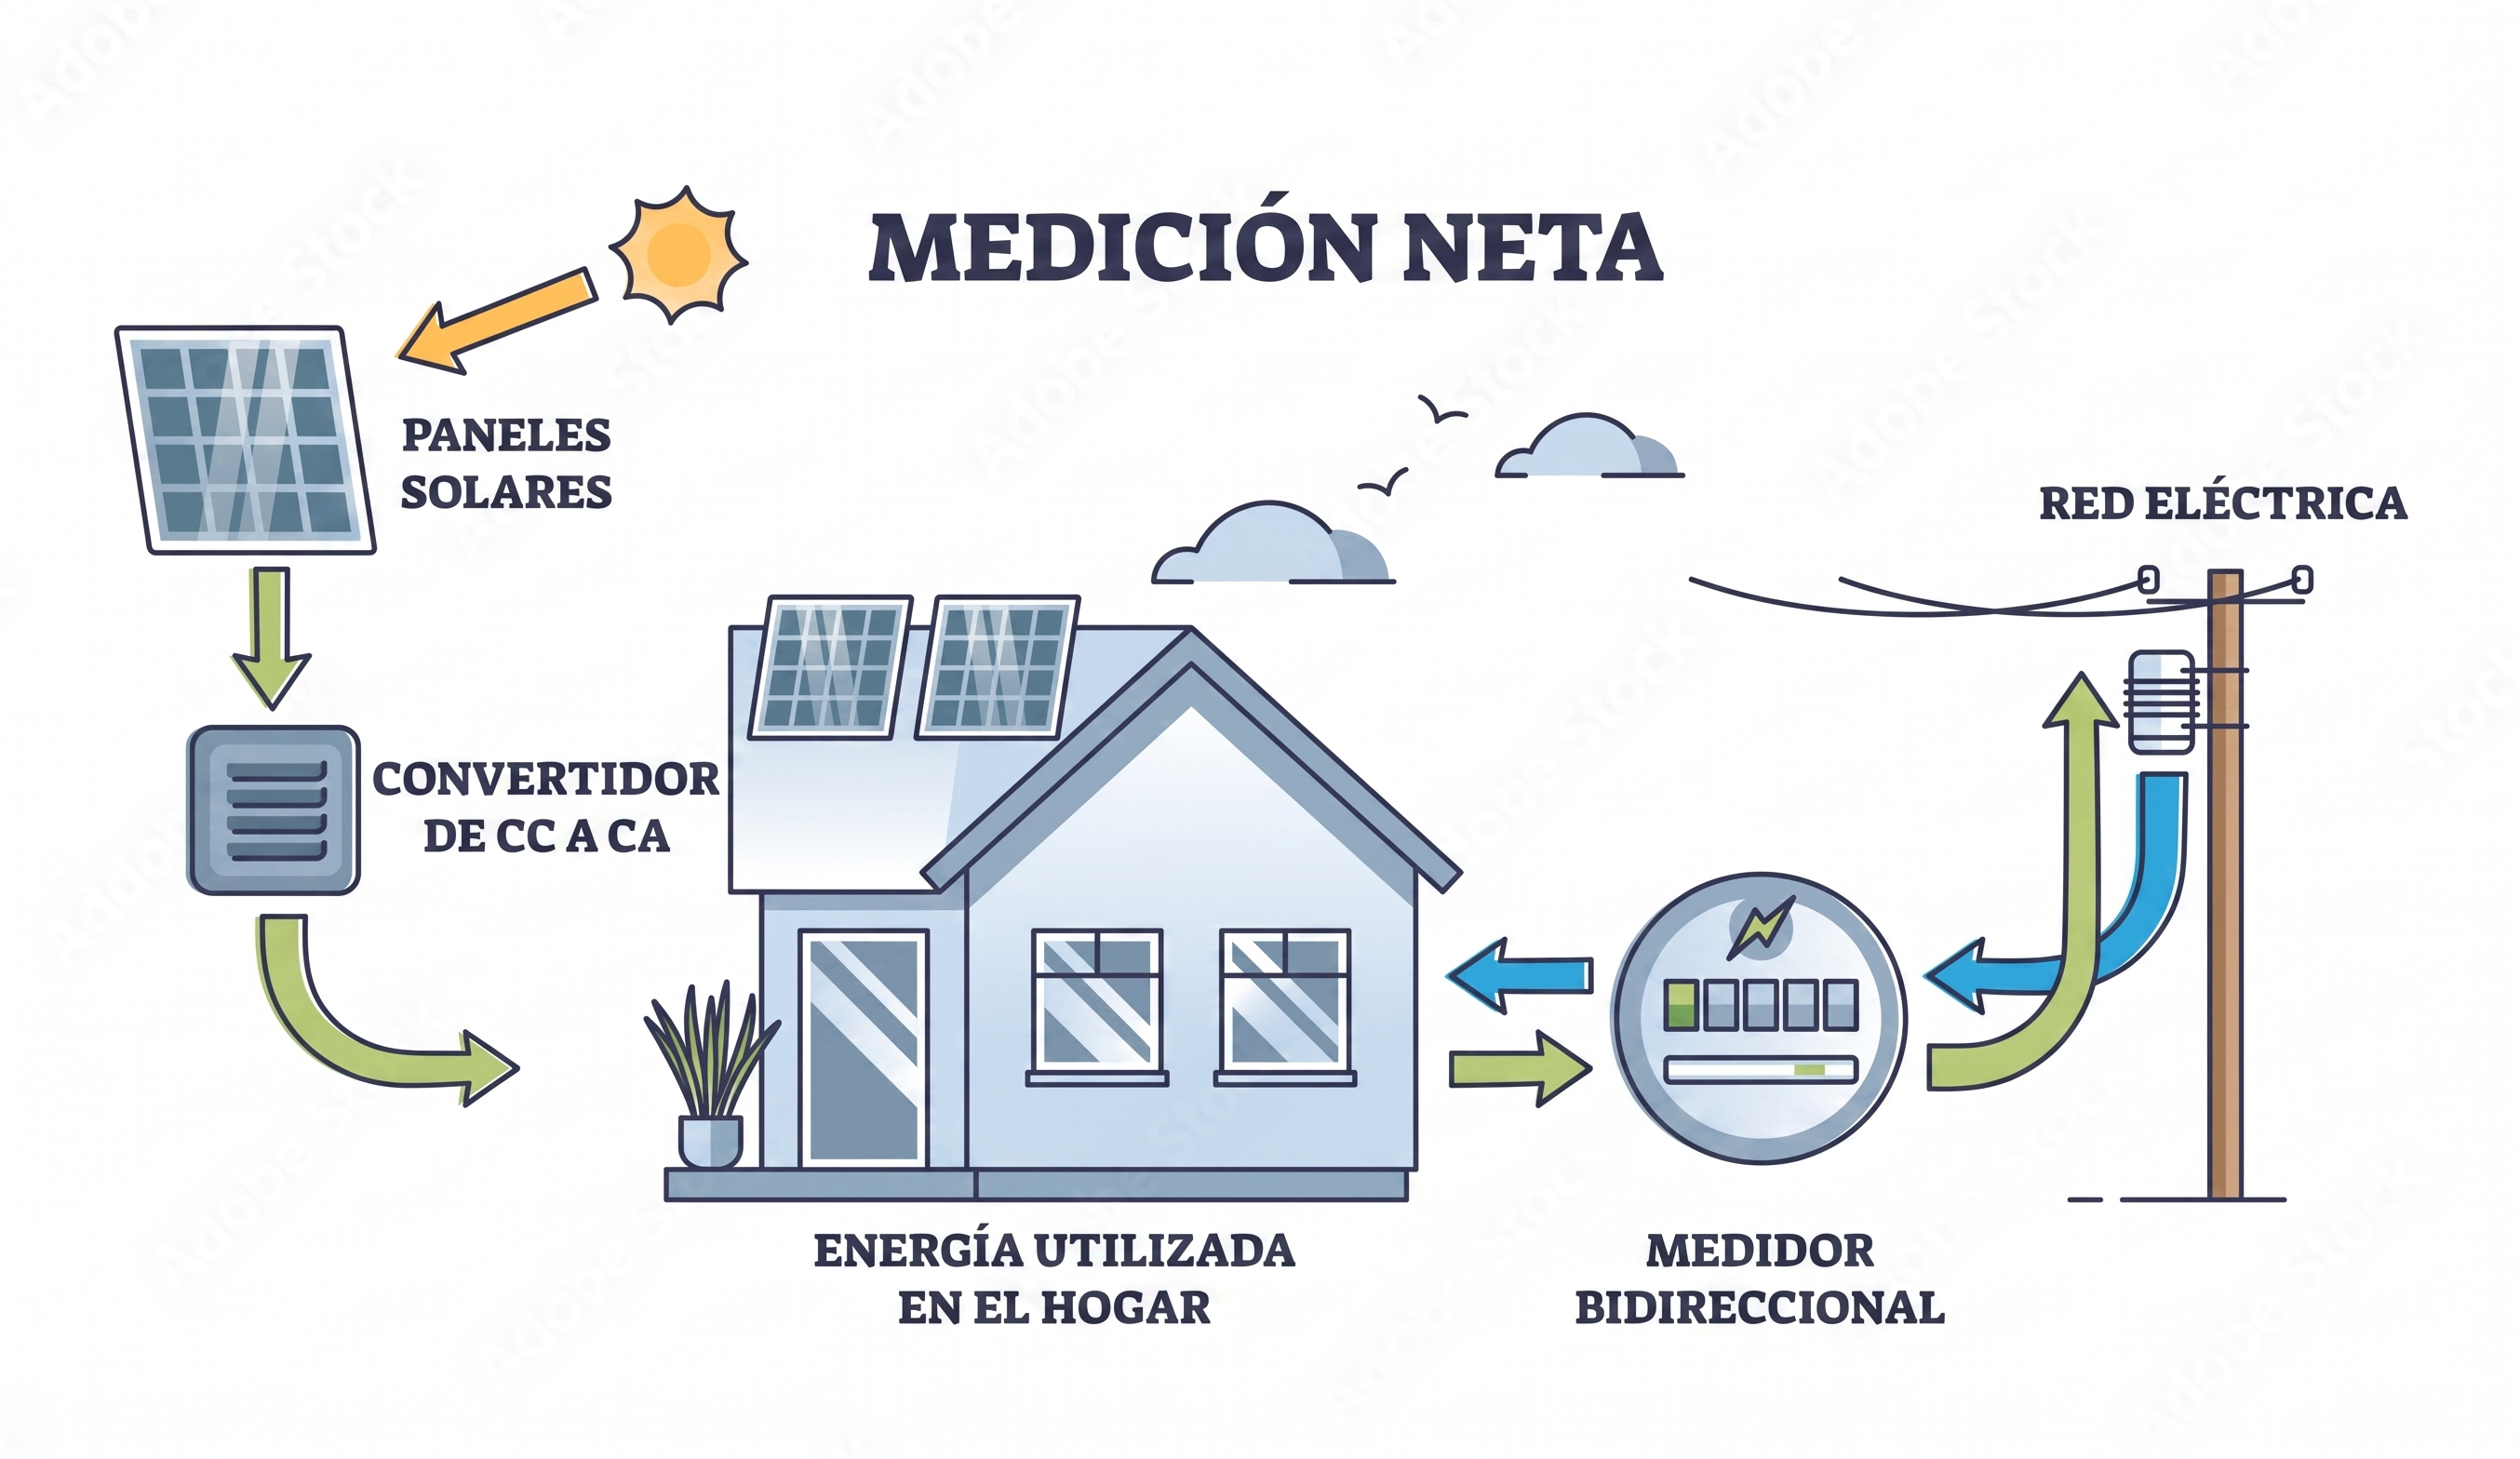
\includegraphics[width=0.85\textwidth]{imgs/diagrama_net_load.png}
  \caption{Medición de carga neta entre red e instalación.}
  \label{fig:net_load_concept}
\end{figure}


\subsection{Diseño de Hardware}

\subsubsection{Selección de Componentes}

La elección de los microcontroladores centrales se basó en la división de tareas entre la adquisición de datos de alta velocidad y la gestión de comunicaciones:

\begin{itemize}
  \item \textbf{STM32F103 (Núcleo de Medición):} Seleccionado por su arquitectura ARM Cortex-M3 de 32 bits \cite{st_rm0008}. Una ventaja tecnológica crucial de este modelo es la integración de dos unidades de ADC independientes. Esta característica permite configurar el modo de \textit{muestreo simultáneo}, capturando en el mismo instante de tiempo la señal de tensión y la de corriente correspondientes a una fase. Esta sincronización es fundamental para evitar errores en el cálculo de la potencia activa, reactiva y el factor de potencia, los cuales son extremadamente sensibles a cualquier desfasaje temporal introducido por el hardware de adquisición.
  \item \textbf{ESP32-C3 (Gateway IoT):} Seleccionado por su bajo costo, su reducido factor de forma (\textit{footprint}) y su alta disponibilidad en el mercado \cite{esp32c3_ds}. Además de su arquitectura RISC-V y periféricos de seguridad, su conectividad nativa Wi-Fi y Bluetooth lo posicionan como una solución óptima para actuar como puente hacia la infraestructura en la nube sin elevar el costo final del dispositivo.
  \item \textbf{MCP4131 (Potenciómetros Digitales):} Utilizados para implementar el sistema de \textit{auto-ranging} de corriente \cite{mcp4131_ds}, permitiendo ajustar la ganancia de los amplificadores de transimpedancia de forma dinámica mediante el bus SPI.
  \item \textbf{LMV324 (Amplificadores Operacionales):} Seleccionados por su capacidad de salida \textit{Rail-to-Rail} y su bajo costo \cite{lmv324_ds}, utilizados en las etapas de acondicionamiento de señal para escalar y desplazar las lecturas de los sensores al rango dinámico del ADC (0-3.3V).
  \item \textbf{ZMPT101B (Sensor de Tensión):} Transformador de tensión activo de bajo costo, capaz de medir niveles de tensión AC comerciales (hasta 250V RMS), cumpliendo con los rangos operativos requeridos para el monitoreo residencial e industrial ligero \cite{zmpt101b_ds}.
  \item \textbf{SCT-013 (Sensor de Corriente):} Transformador de corriente de núcleo partido (\textit{split-core}) que permite una instalación no invasiva \cite{sct013_ds}. Su capacidad de medición de hasta 70A RMS se alinea perfectamente con los objetivos de costo y prestaciones definidos por la empresa para este medidor.

  \item \textbf{HLK-5M05 (Etapa de Alimentación Interna):} El dispositivo integra la fuente conmutada \textbf{HLK-5M05} \cite{hlk5m05_ds} que permite su funcionamiento autónomo mediante la toma de energía directa de la Fase~1 de la red eléctrica, simplificando significativamente el proceso de instalación al prescindir de fuentes externas.
\end{itemize}

\subsubsection{Acondicionamiento de Señal y Auto-ranging}

Para maximizar la precisión en un amplio espectro de potencias, se implementó una etapa de acondicionamiento de señal activa con capacidad de ajuste de rango automático (\textit{auto-ranging}). Esta estrategia es fundamental para resolver el compromiso tecnológico entre la resolución necesaria para medir cargas pequeñas y el rango dinámico requerido para potencias elevadas.

El sistema utiliza potenciómetros digitales \textbf{MCP4131} \cite{mcp4131_ds} integrados en la etapa de realimentación de los amplificadores operacionales \textbf{LMV324}. El firmware del STM32F103 monitorea continuamente los valores de pico de la señal de corriente en cada fase. Si la amplitud de la señal cae por debajo de un umbral predefinido, el microcontrolador incrementa la ganancia del amplificador mediante el bus SPI, permitiendo que señales pequeñas ocupen una mayor porción del rango del ADC (\SI{0}{\volt} a \SI{3.3}{\volt}). Inversamente, ante un incremento de la carga que amenace con saturar el ADC, el sistema reduce la ganancia de forma inmediata para evitar el truncamiento (\textit{clipping}) de la forma de onda.


Gracias a esta implementación de \textit{auto-ranging}, el dispositivo logra una excelente linealidad y precisión incluso en consumos inferiores a los \SI{500}{\watt}, manteniendo la capacidad de registrar picos de demanda de hasta \SI{17.5}{\kilo\watt}. Esto dota al medidor de una versatilidad excepcional, siendo capaz de capturar desde el consumo residual de equipos en \textit{standby} hasta el flujo energético completo de una instalación residencial o comercial pesada. Esta característica representa una ventaja competitiva frente a soluciones comerciales consolidadas \cite{shelly_pro_3em}, que por limitaciones de diseño suelen aplicar zonas muertas (\textit{deadbands}) que ignoran consumos por debajo de ciertos umbrales de corriente, perdiendo así información sobre el consumo de la instalación.



\subsubsection{Etapa de Comunicaciones y Gateway}

\subsubsection{Diseño del Esquema Eléctrico y Circuito Impreso (PCB)}

Para la integración física de los componentes y la validación del prototipo, se diseñó un circuito impreso (PCB) utilizando la herramienta de diseño electrónico automatizado (EDA) \textbf{KiCad}.


\begin{figure}[htbp]
  \centering
  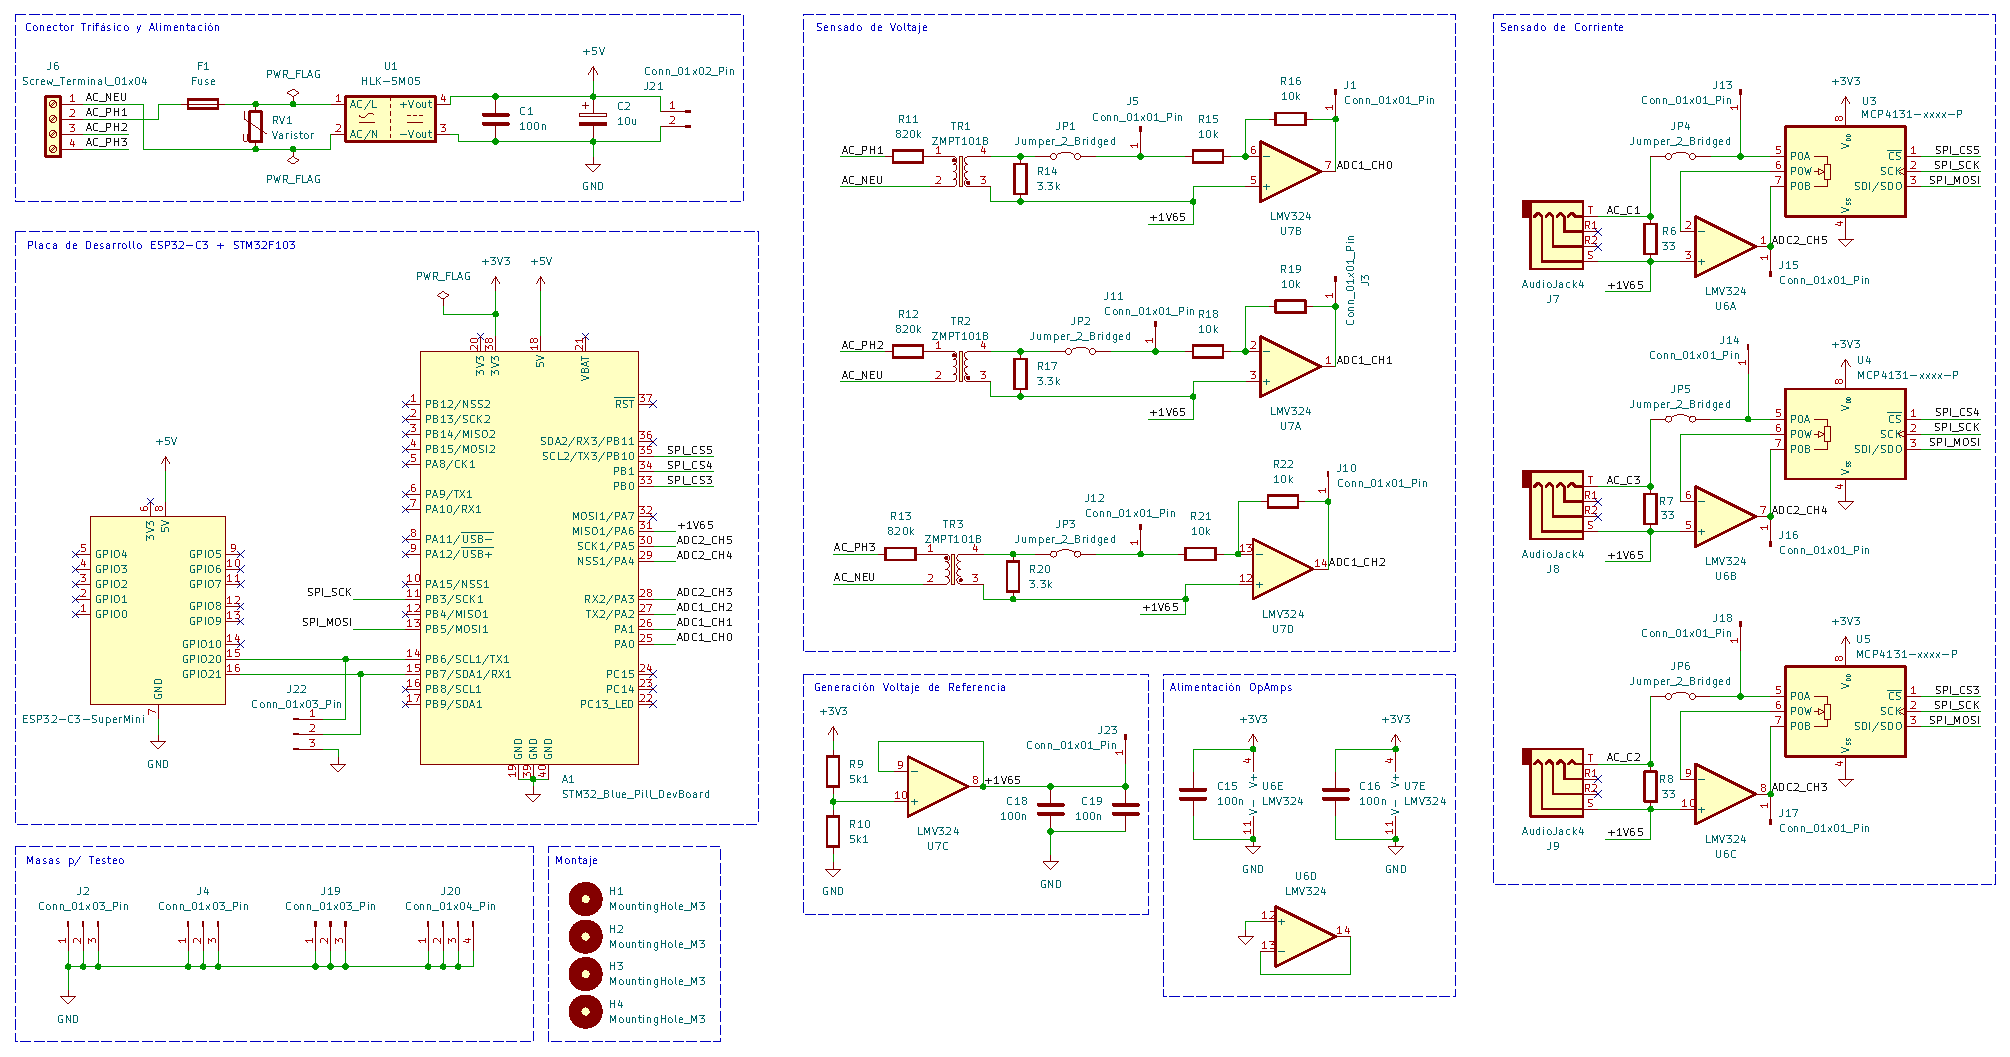
\includegraphics[width=\textwidth]{imgs/esquematico_kicad.pdf}
  \caption{Diagrama esquemático del sistema de medición y gateway.}
  \label{fig:pcb_schematic}
\end{figure}

En el Anexo \ref{sec:anexo_pcb} se presentan capturas adicionales del diseño, incluyendo el ruteado de pistas y vistas 3D de la placa.

\subsection{Caracterización y Ensayo de Sensores}

El desempeño del medidor está íntimamente ligado a la respuesta de los sensores de tensión y corriente. Para ambos sensores, el \textbf{SCT-013} y el \textbf{ZMPT101B}, sus hojas de datos incorporan información suficiente para conocer sus linealidades dentro del rango de carga de interés para este proyecto. Sin embargo, se identificó que era necesario un estudio con mayor detenimiento para caracterizar con precisión los retardos de fase introducidos por los sensores y sus respectivos circuitos de acondicionamiento, ya que estos son críticos para el cálculo de la potencia activa y el factor de potencia.

\subsubsection{Metodología}

Con el objetivo de validar la respuesta del sistema ante diferentes condiciones de carga y tipos de señal, se llevó a cabo una etapa de ensayos utilizando una fuente de tensión alterna de \SI{220}{\volt} y variando la corriente de carga. Los ensayos se dividieron en dos escenarios principales:

\begin{itemize}
  \item \textbf{Escenario 1: Señal Senoidal Pura.} Se evaluó el desempeño con corrientes de \SI{10}{\ampere} y \SI{20}{\ampere}, manteniendo un factor de potencia unitario ($PF=1$) y un factor de cresta de 3 ($CF=3$). Se probaron configuraciones con la referencia del ADC centrada en \SI{1.65}{\volt} y referenciada a masa (GND).
  \item \textbf{Escenario 2: Señal Distorsionada.} Se aplicó una tensión de \SI{220}{\volt} con distorsión armónica y una carga de \SI{15}{\ampere} (con un ángulo de fase de $0^\circ$).
\end{itemize}

Para caracterizar con precisión el retardo de fase introducido por los sensores y sus etapas de acondicionamiento, se empleó una metodología basada en la \textbf{Transformada de Hilbert}. Esta técnica permite obtener la señal analítica de las capturas temporales, facilitando el cálculo de la fase instantánea de cada señal.

A diferencia de los métodos convencionales basados en la detección de cruces por cero, que pueden ser sensibles al ruido o a pequeñas distorsiones armónicas, la Transformada de Hilbert proporciona una medición continua del desfase a lo largo de todo el periodo de la señal. Mediante este análisis, se determinó la diferencia de fase promedio entre la señal de referencia de la fuente y la señal capturada por el sistema, permitiendo compensar estos retardos en el firmware para mejorar la precisión del cálculo de potencia activa.
Las figuras~\ref{fig:hilbert_phase_voltage}, \ref{fig:hilbert_signals_current}
y~\ref{fig:hilbert_comparacion} ilustran el análisis para un caso representativo de los
ensayos realizados; el diagrama de caja de la figura~\ref{fig:boxplot_ensayo} consolida los
resultados del conjunto completo de ensayos.

\begin{figure}[htbp]
  \centering
  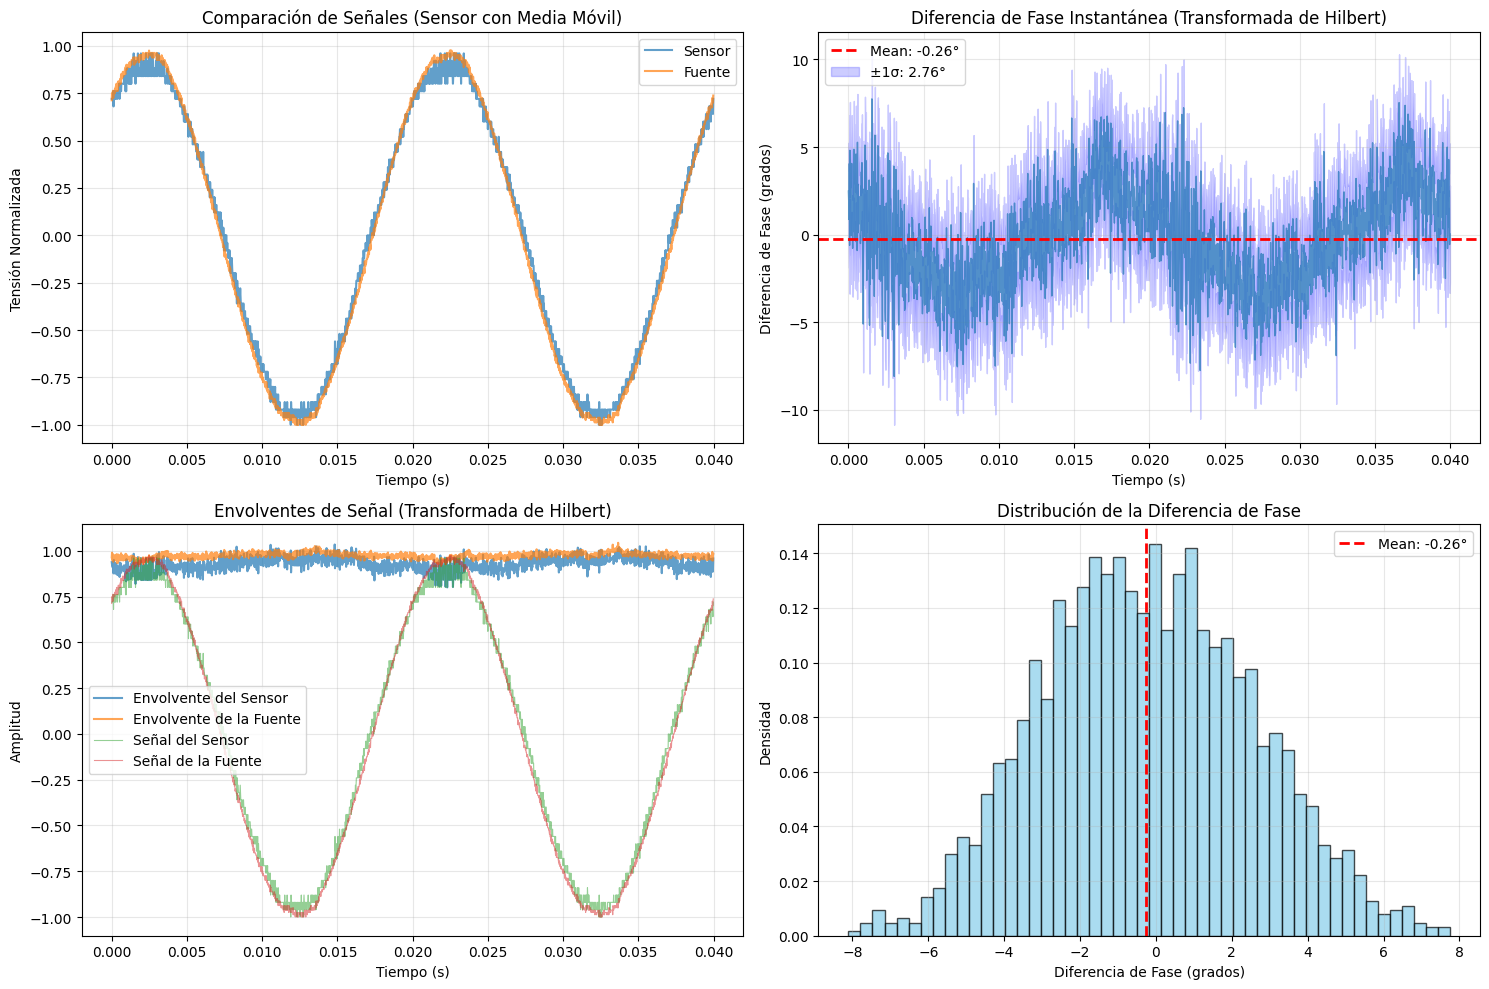
\includegraphics[width=0.8\textwidth]{imgs/plots_voltaje.png}
  \caption{Caracterización de desfase del sensor de tensión ZMPT101B.}
  \label{fig:hilbert_phase_voltage}
\end{figure}

\begin{figure}[htbp]
  \centering
  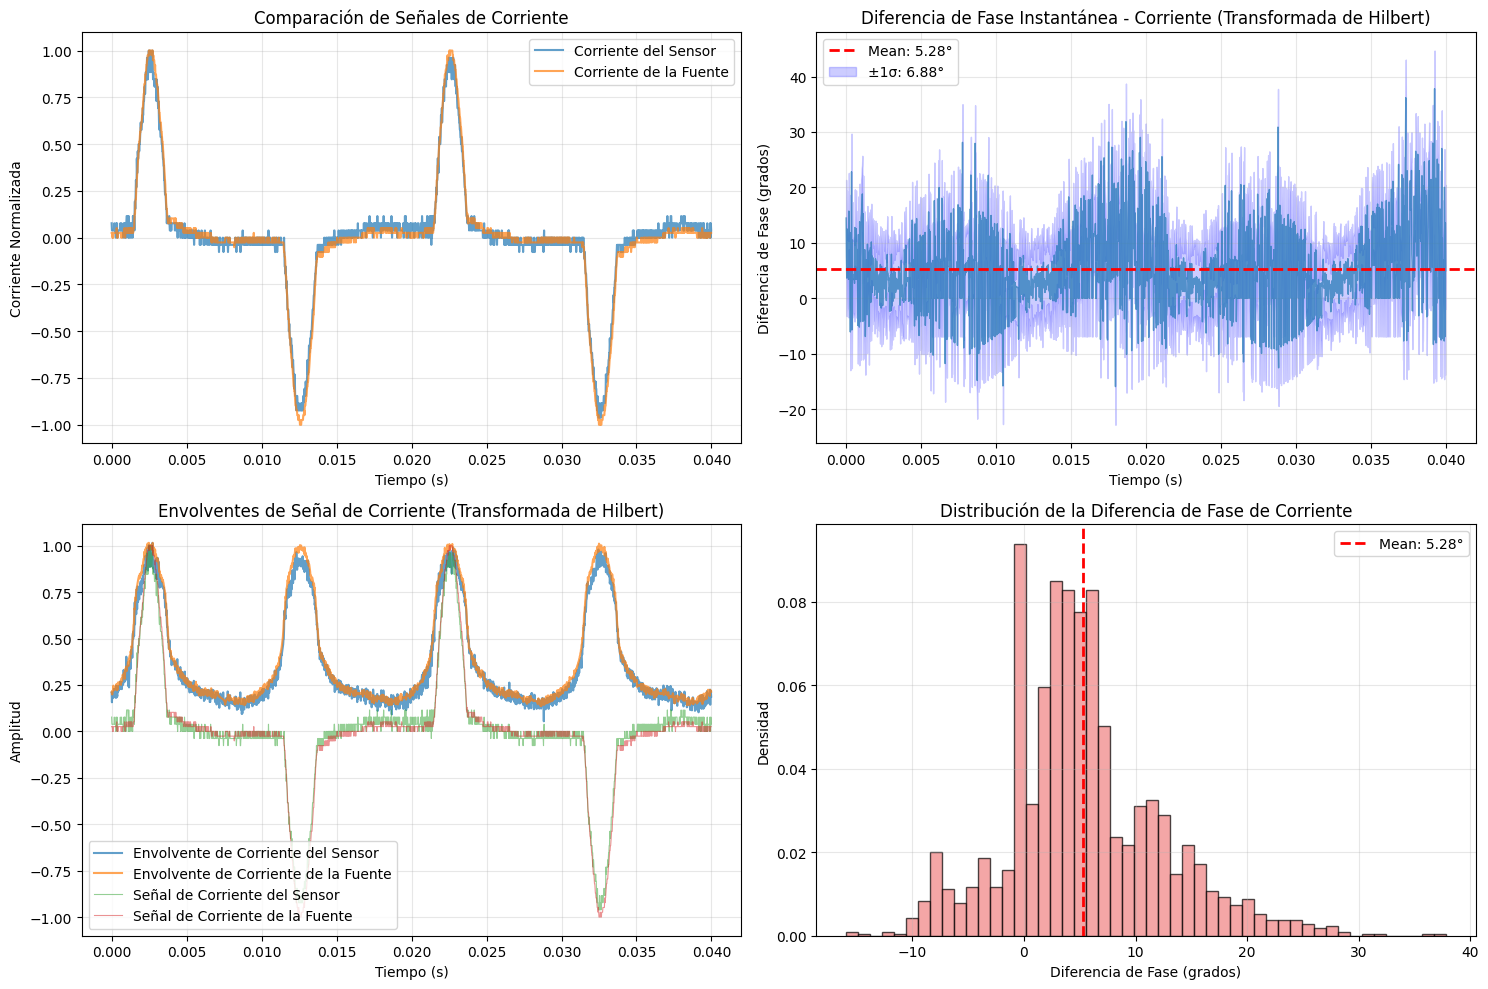
\includegraphics[width=0.8\textwidth]{imgs/plots_corriente.png}
  \caption{Caracterización de desfase del sensor de corriente SCT-013.}
  \label{fig:hilbert_signals_current}
\end{figure}

\begin{figure}[htbp]
  \centering
  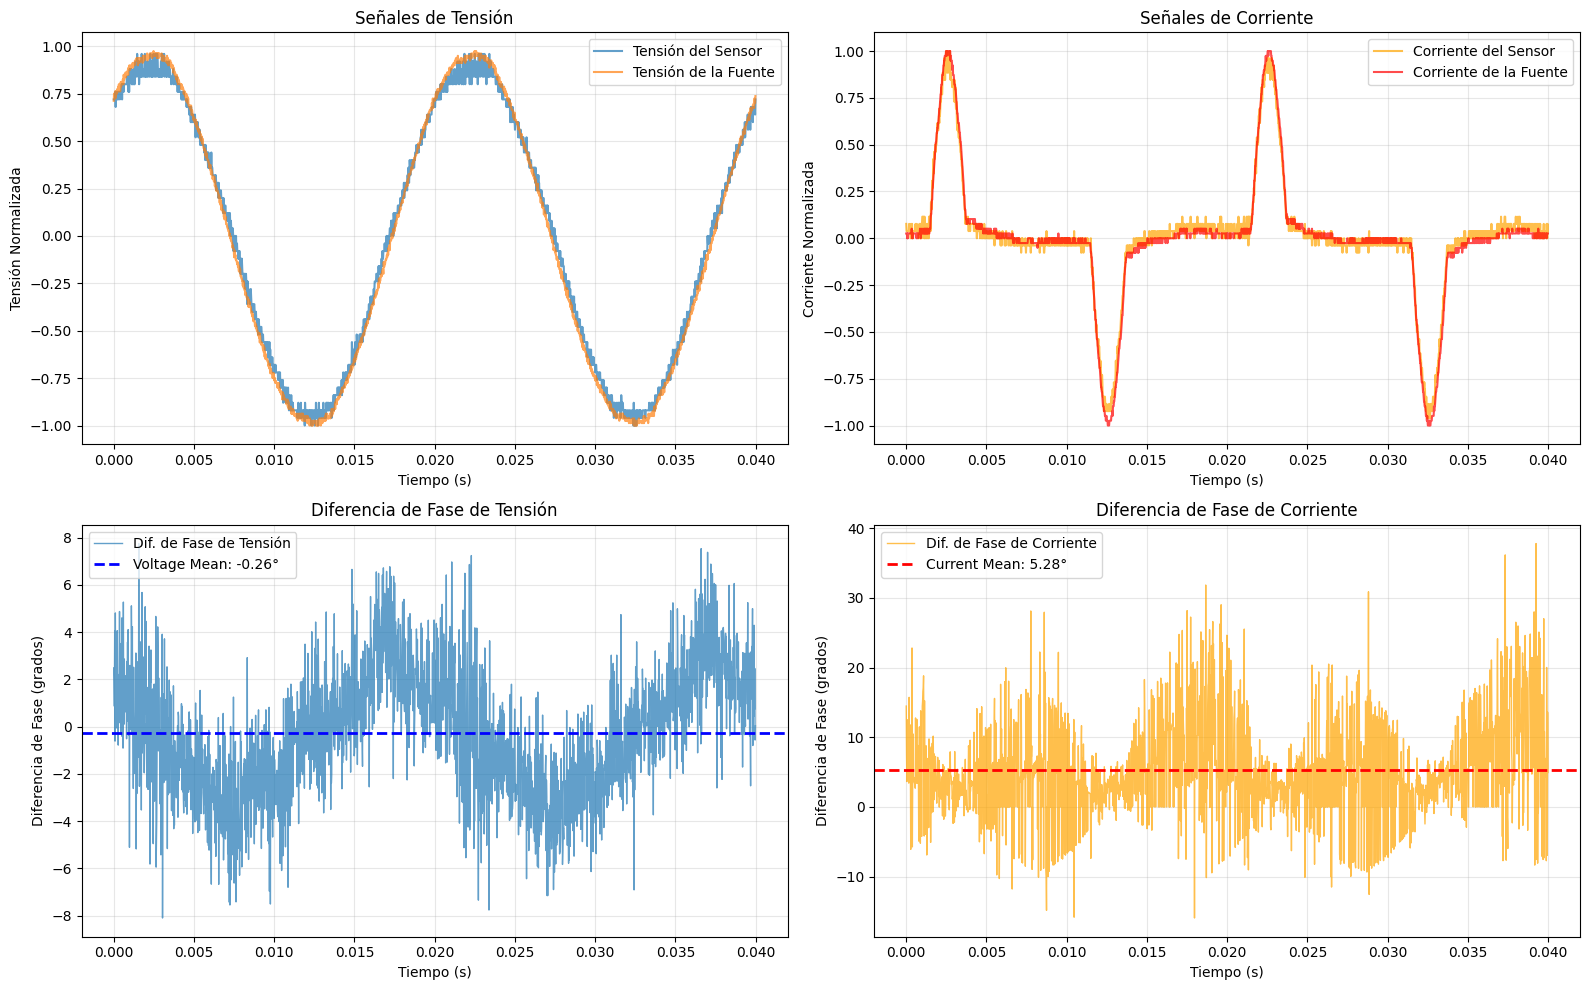
\includegraphics[width=0.8\textwidth]{imgs/plots_comparacion.png}
  \caption{Comparación de señales y diferencias de fase para ambos sensores.}
  \label{fig:hilbert_comparacion}
\end{figure}

\begin{figure}[htbp]
  \centering
  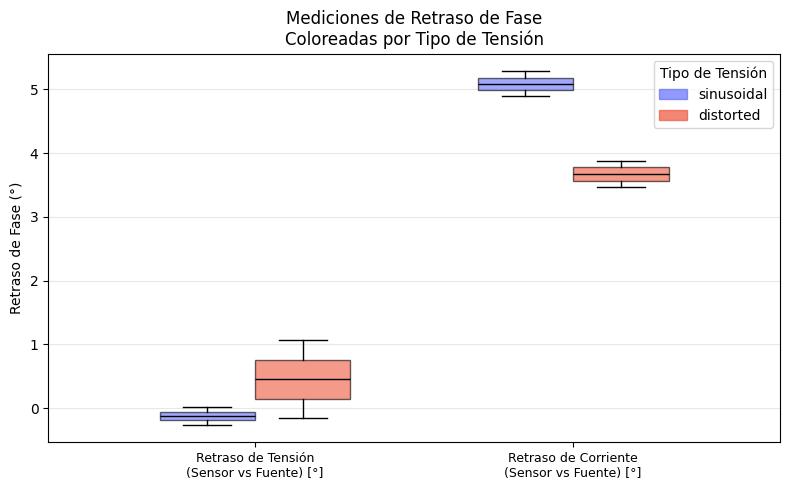
\includegraphics[width=0.8\textwidth]{imgs/plots_ensayo.png}
  \caption{Diagrama de caja del desfase medido, agrupado por tipo de señal de tensión.}
  \label{fig:boxplot_ensayo}
\end{figure}

\subsubsection{Resultados}

El análisis mediante Transformada de Hilbert sobre los datos adquiridos en los ensayos permitió
cuantificar con precisión los retardos de fase introducidos por cada sensor y su etapa de
acondicionamiento. Las figuras~\ref{fig:hilbert_phase_voltage} y~\ref{fig:hilbert_signals_current}
muestran, para un caso particular de los ensayos, los cuatro paneles del análisis:
la comparación de señales normalizadas, la diferencia de fase instantánea con banda de
$\pm1\sigma$, las envolventes analíticas y la distribución estadística del desfase,
respectivamente para el ZMPT101B y el SCT-013. La
figura~\ref{fig:hilbert_comparacion} presenta ambos sensores de forma simultánea para facilitar
la comparación directa. Los resultados que se presentan a continuación reflejan los promedios
obtenidos sobre el conjunto completo de ensayos:

\begin{itemize}
  \item \textbf{Sensor de Tensión ZMPT101B:} El desfase promedio medido entre la referencia
        de la fuente y la señal del sensor resultó de $\bar{\phi} = 0{,}16^\circ$, con una
        desviación estándar de $\sigma = 0{,}61^\circ$. El valor medio prácticamente nulo indica
        que el transformador ZMPT101B introduce un retardo de fase despreciable a la frecuencia
        de red de 50 Hz.

  \item \textbf{Sensor de Corriente SCT-013:} El desfase promedio fue de $\bar{\phi} = 4{,}38^\circ$,
        con una desviación estándar de $\sigma = 0{,}85^\circ$. Este retardo es un valor conocido,
        determinístico y bien caracterizado bajo las condiciones de ensayo, lo que permite
        compensarlo en el firmware del STM32F103 para garantizar el cálculo correcto de potencia
        activa y factor de potencia.
\end{itemize}

En el diagrama de caja de la figura~\ref{fig:boxplot_ensayo} se aprecia la diferencia
de comportamiento según el tipo de señal: bajo señal senoidal el ZMPT101B presenta un desfase
cercano a $-0{,}1^\circ$, mientras que con señal distorsionada se desplaza hacia $\approx 0{,}5^\circ$.
El SCT-013, por su parte, mantiene un retardo de $\approx 5{,}1^\circ$ bajo señal senoidal y
desciende a $\approx 3{,}7^\circ$ con señal distorsionada, confirmando la estabilidad general
del sensor en ambos escenarios.




\subsection{Implementación del Firmware}

\subsubsection{Cómputo de Variables Eléctricas (STM32F103)}

El núcleo de medición se basa en un STM32F103 que ejecuta un bucle de procesamiento en tiempo real. Los aspectos más destacados de su implementación incluyen:

\begin{itemize}
  \item \textbf{Muestreo Sincronizado:} Se utiliza el temporizador \texttt{TIM3} para disparar la conversión del ADC a una frecuencia de 5 kHz por canal. La adquisición se realiza mediante DMA para minimizar la carga de la CPU.
  \item \textbf{Sincronización de Fase:} El sistema detecta los cruces por cero de la tensión en la fase 1 (utilizando un esquema de histéresis) para definir el inicio y fin de cada ciclo de red (50 Hz). Esto permite realizar integraciones precisas sobre periodos completos.
  \item \textbf{Cálculos Eléctricos:} Para cada ciclo, se calculan los valores eficaces (RMS) y la potencia activa mediante la suma de los productos instantáneos de tensión y corriente.
  \item \textbf{Sistema de Rango Automático (\textit{Auto-ranging}):} Mediante potenciómetros digitales MCP4131 controlados por SPI, el firmware monitorea los valores pico de corriente. Si la señal se aproxima a la saturación o es demasiado pequeña, el sistema ajusta dinámicamente la ganancia del amplificador de transimpedancia, garantizando la máxima resolución del ADC en todo el rango de operación.
\end{itemize}

\subsubsection{Gateway IoT y Seguridad (ESP32-C3)}

El ESP32-C3 actúa como puente entre el hardware de medición y la infraestructura en la nube. Sus funciones principales son:

\begin{itemize}
  \item \textbf{Gestión de Conectividad:} Utiliza la librería \textit{WiFiManager} para permitir al usuario configurar las credenciales de red mediante un portal cautivo, evitando la necesidad de hardcodear datos de acceso.
  \item \textbf{Seguridad en la Transmisión:} La comunicación con el servidor se realiza mediante el protocolo MQTTS \cite{mqtt_spec}. Se integra el certificado raíz de \textit{Let's Encrypt} para validar la identidad del broker y establecer un túnel cifrado TLS 1.2.

  \item \textbf{Intercambio de Datos:} Recibe tramas JSON desde el STM32 vía UART, las procesa para añadir metadatos de diagnóstico y las publica en tópicos MQTT estructurados por la dirección MAC del dispositivo.
  \item \textbf{Diagnóstico Local:} Implementa un sistema de \textit{logging} persistente en la memoria flash (\textit{LittleFS}), accesible a través de una interfaz web interna.
  \item \textbf{Resolución de Nombres (mDNS):} Soporta el protocolo de red \textit{multicast DNS}, permitiendo que los usuarios accedan a la interfaz de configuración mediante el nombre de dominio local \texttt{enerlab.local}, facilitando el acceso sin necesidad de conocer la dirección IP asignada por el router.
\end{itemize}

\subsubsection{Portal Captivo y Monitoreo Local}

El dispositivo implementa una interfaz de configuración y monitoreo local accesible vía Wi-Fi, lo que facilita la puesta en marcha y el diagnóstico en campo sin necesidad de herramientas externas:

\begin{figure}[htbp]
  \centering
  \begin{subfigure}[b]{0.45\textwidth}
    \centering
    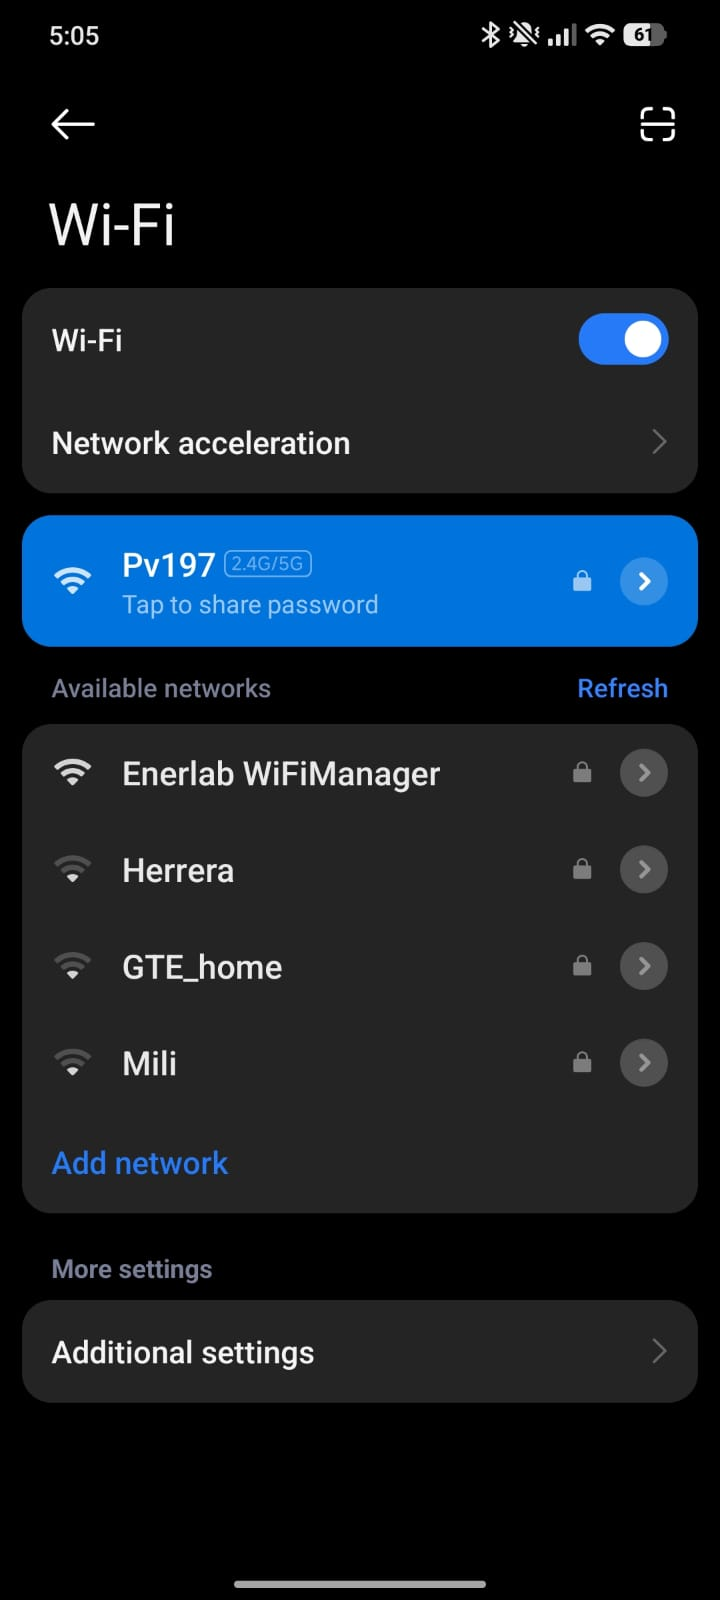
\includegraphics[height=9cm]{imgs/portal_1.jpeg}
    \caption{Red Wi-Fi generada por el dispositivo.}
    \label{fig:portal_1}
  \end{subfigure}
  \hfill
  \begin{subfigure}[b]{0.45\textwidth}
    \centering
    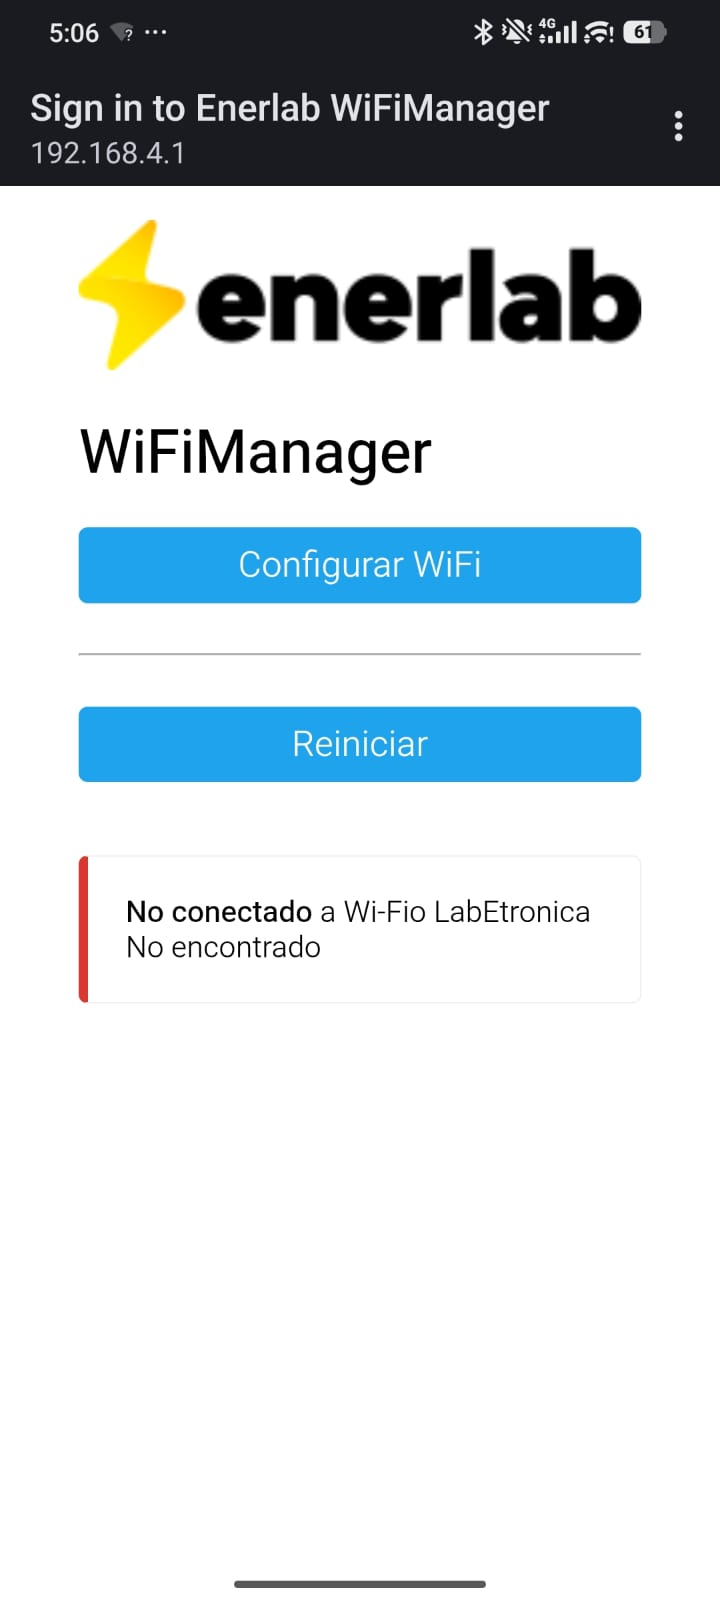
\includegraphics[height=9cm]{imgs/portal_2.jpeg}
    \caption{Portal captivo detectado al conectar.}
    \label{fig:portal_2}
  \end{subfigure}
  \\[2ex]
  \begin{subfigure}[b]{0.45\textwidth}
    \centering
    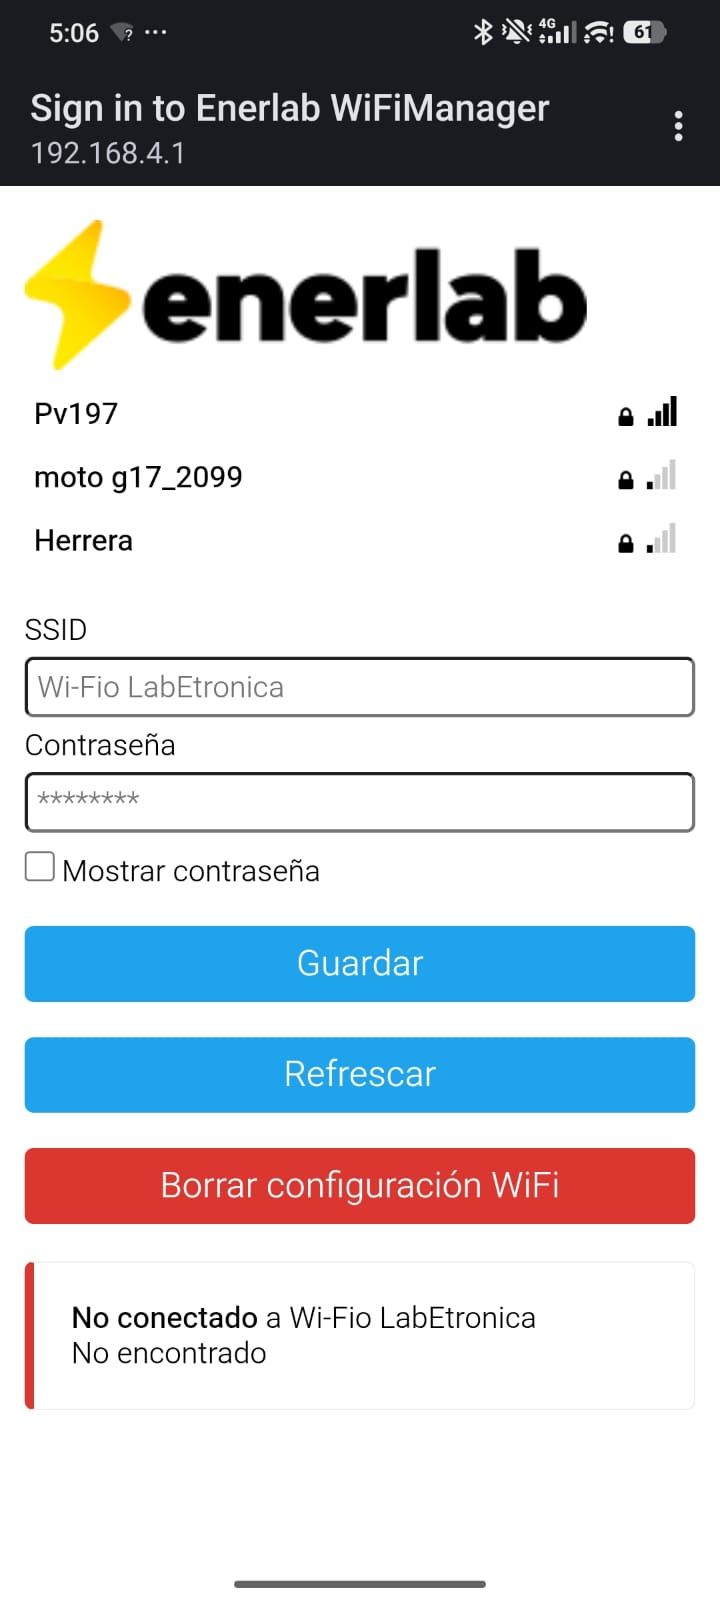
\includegraphics[height=9cm]{imgs/portal_3.jpeg}
    \caption{Formulario de configuración y escaneo.}
    \label{fig:portal_3}
  \end{subfigure}
  \hfill
  \begin{subfigure}[b]{0.45\textwidth}
    \centering
    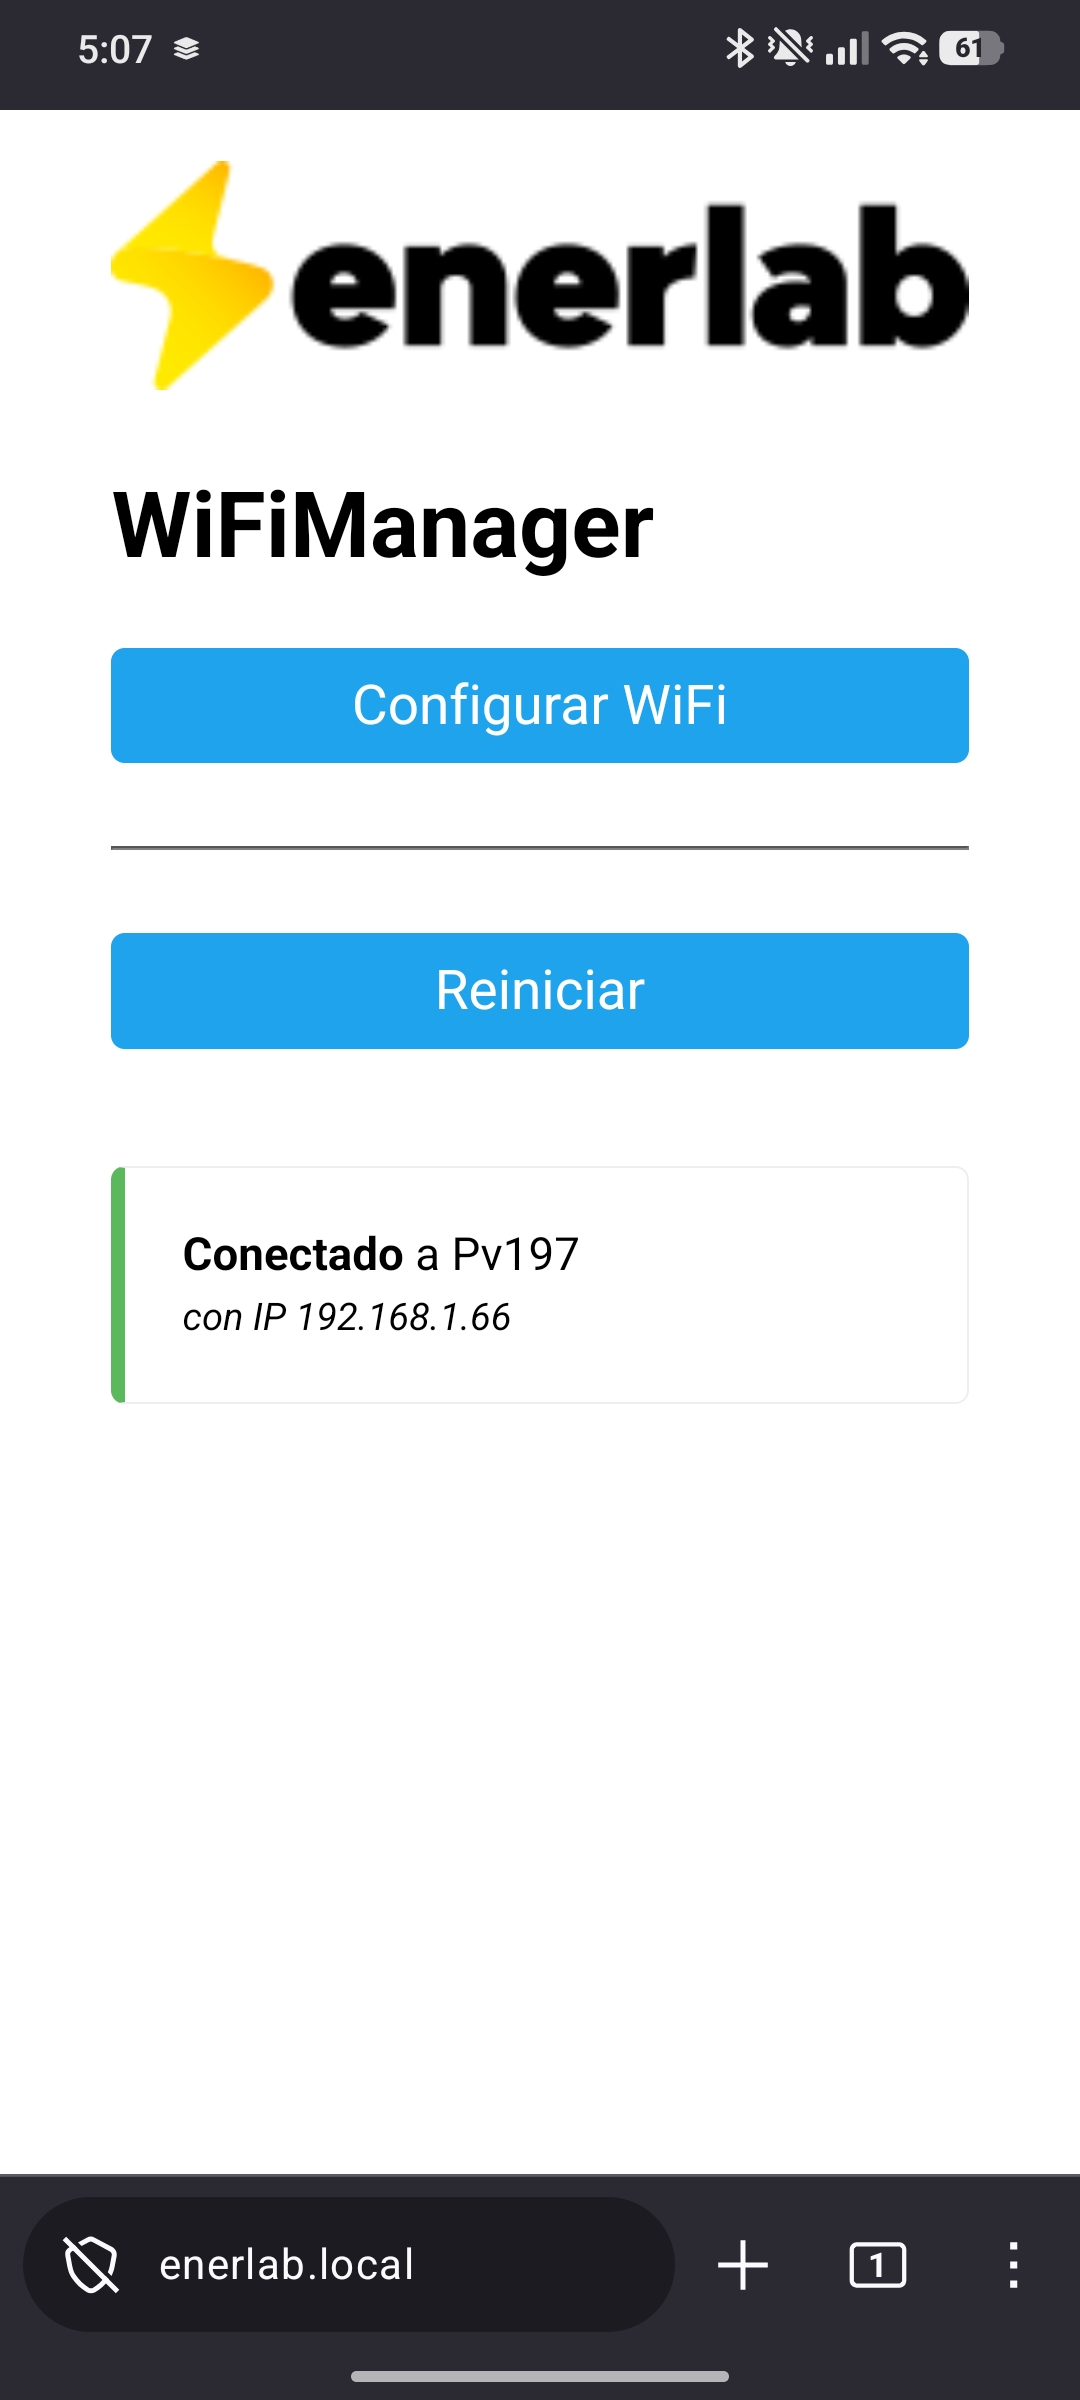
\includegraphics[height=9cm]{imgs/portal_4.jpeg}
    \caption{Confirmación de conexión exitosa.}
    \label{fig:portal_4}
  \end{subfigure}
  \caption{Proceso de configuración inicial de Wi-Fi mediante el portal captivo.}
  \label{fig:portal_wifi_config}
\end{figure}

\begin{itemize}
  \item \textbf{Portal Captivo de Configuración:} Utilizando la librería \textit{WiFiManager}, el ESP32 es capaz de detectar la falta de conectividad y activar un modo de Punto de Acceso (AP) con un portal captivo. Este portal permite al usuario seleccionar la red Wi-Fi local e ingresar las credenciales sin que estas queden grabadas de forma estática en el código fuente. La interfaz ha sido personalizada con el logotipo del proyecto y un menú simplificado. En la figura~\ref{fig:portal_wifi_config} se ilustran los pasos de este proceso.
  \item \textbf{Panel de Monitoreo y Herramientas:} Una vez establecida la conexión, el gateway sirve una interfaz web accesible mediante \texttt{enerlab.local}. Esta permite visualizar el estado de la conexión MQTT, las versiones de firmware de ambos microcontroladores y realizar acciones de mantenimiento como el reinicio remoto del dispositivo (ver figura~\ref{fig:portal_info}).
  \item \textbf{Visualización de Logs:} A través de la ruta \texttt{/logs}, el servidor web del ESP32 entrega el contenido del archivo de registro almacenado en \textit{LittleFS}, permitiendo una depuración rápida de problemas de red o comunicación con el STM32 (ver figura~\ref{fig:portal_logs}).
\end{itemize}

\begin{figure}[htb]
  \centering
  \begin{subfigure}[b]{0.45\textwidth}
    \centering
    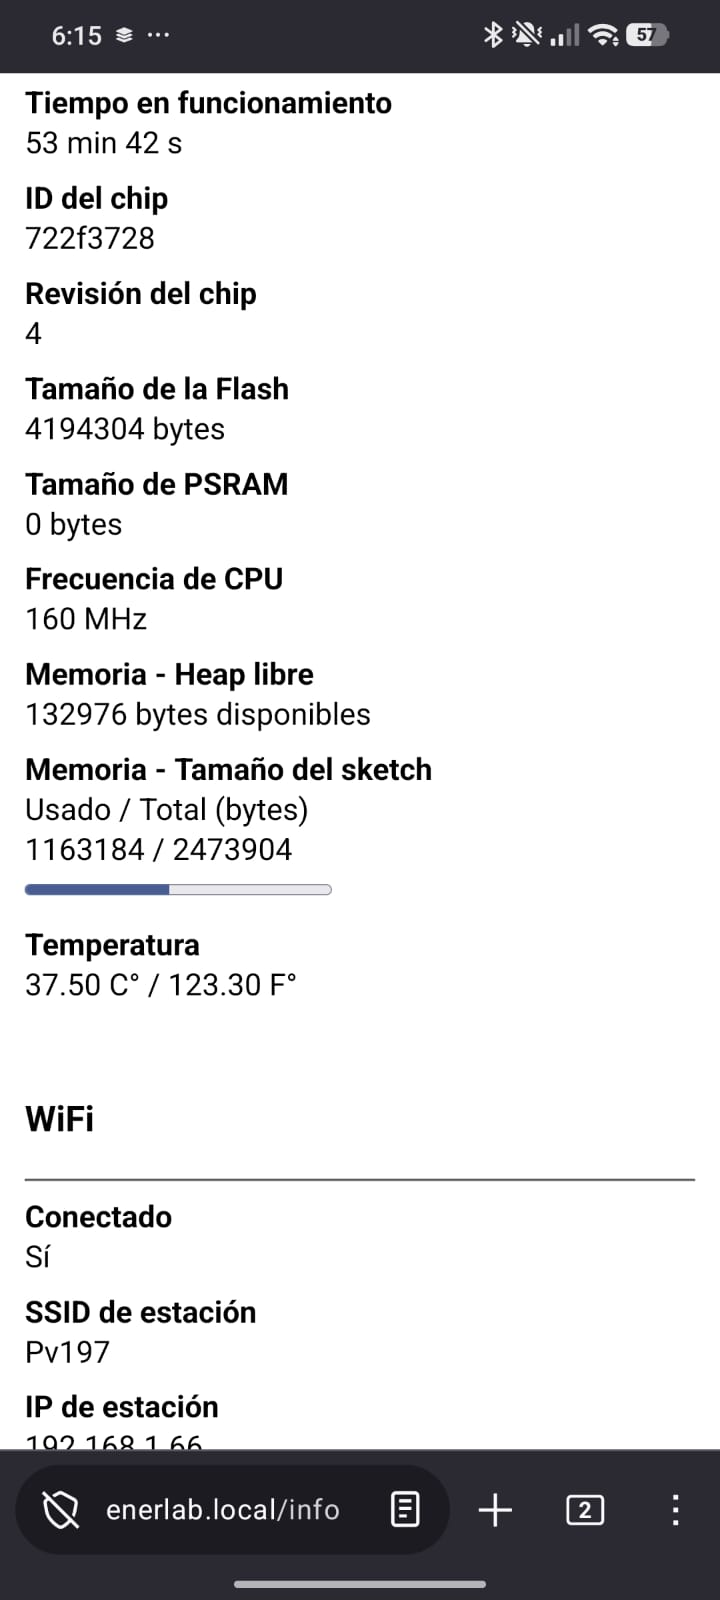
\includegraphics[height=9cm]{imgs/portal_info.jpeg}
    \caption{Estado del sistema y conexión.}
    \label{fig:portal_info}
  \end{subfigure}
  \hfill
  \begin{subfigure}[b]{0.45\textwidth}
    \centering
    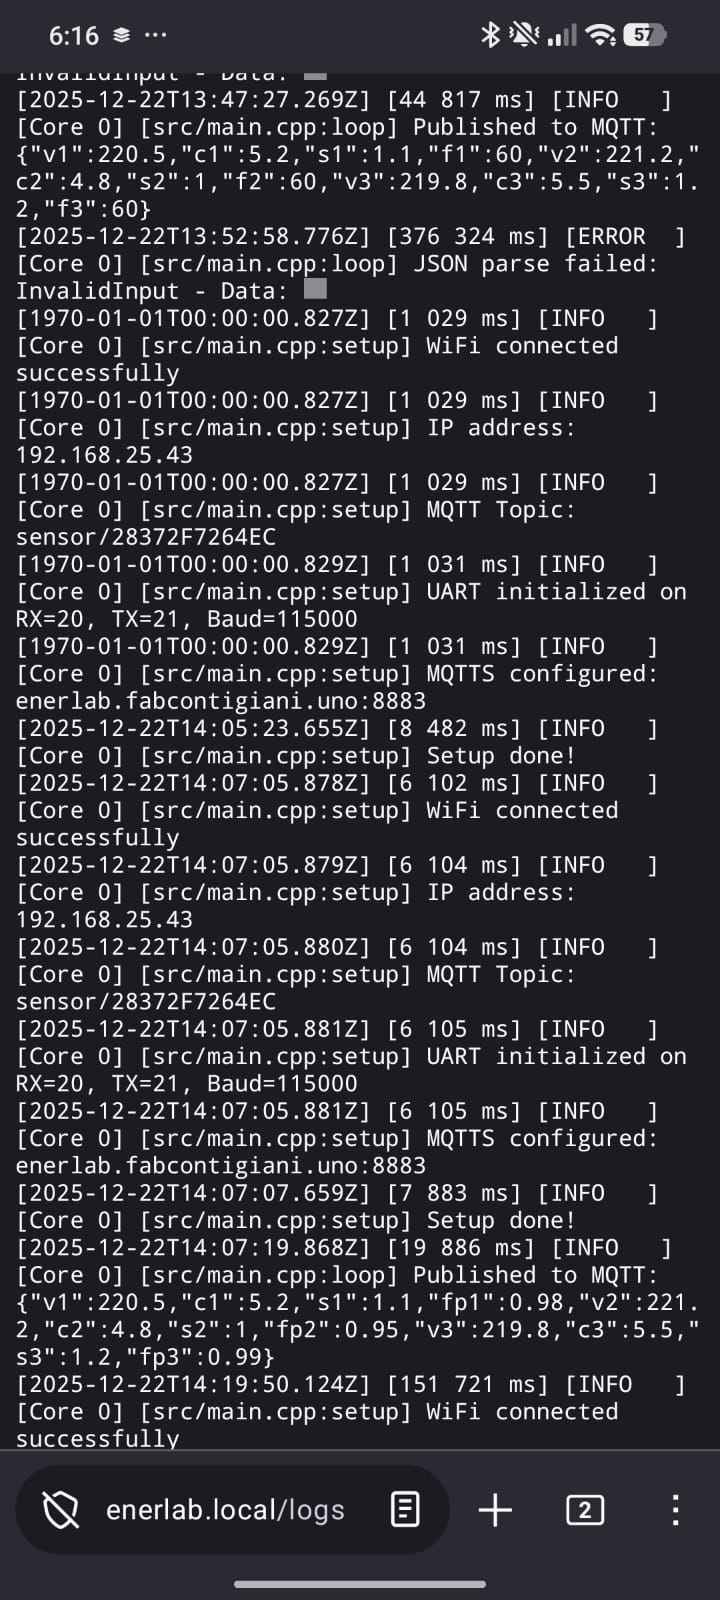
\includegraphics[height=9cm]{imgs/portal_logs.jpeg}
    \caption{Registro de eventos locales.}
    \label{fig:portal_logs}
  \end{subfigure}
  \caption{Interfaz web de monitoreo local y diagnóstico.}
  \label{fig:web_monitoreo}
\end{figure}

\subsection{Interfaz de Usuario y Almacenamiento Remoto}

\subsubsection{Selección y Justificación de la Arquitectura}

Previo a la implementación de los servicios remotos, se realizó un análisis de las posibles arquitecturas para el almacenamiento y visualización de datos:

\begin{itemize}
  \item \textbf{Descentralizada:} Procesamiento y almacenamiento local en el dispositivo (ej. mediante una SBC). Si bien ofrece autonomía, incrementa significativamente el costo del hardware y dificulta el acceso remoto en entornos sin IP pública.
  \item \textbf{Mixta:} Almacenamiento local con acceso remoto vía túneles (SSH/VPN). Requiere infraestructura a medida y mantenimiento complejo.
  \item \textbf{Centralizada (Seleccionada):} Los datos se envían a un servidor remoto (VPS o Nube). Esta opción optimiza el costo del hardware del medidor y centraliza el mantenimiento, facilitando la escalabilidad del sistema.
\end{itemize}

En cuanto a la gestión de los servicios, se evaluaron las opciones \textit{Fully Managed} (servicios en la nube de terceros) frente a \textit{Self-Managed} (servidores propios). Para este prototipo, se optó por una arquitectura \textbf{Centralizada y Self-Managed}, desplegando microservicios mediante contenedores \textbf{Docker} en un VPS. Esta elección permite un control total sobre la soberanía de los datos y una reducción de costos operativos durante la etapa de desarrollo.

No obstante, cabe destacar que la implementación definitiva en un entorno de producción será responsabilidad de la empresa. Será la organización quien, evaluando los recursos disponibles y la inversión proyectada, determine la arquitectura final. Esto incluye la selección de los mecanismos de resguardo y seguridad para la base de datos —la cual puede contener información sensible de los clientes—, garantizando así el cumplimiento de los estándares de protección de datos requeridos por la institución.

La arquitectura de servicios remotos se diseñó bajo un enfoque de microservicios, utilizando contenedores \textbf{Docker} para garantizar la portabilidad y facilitar el despliegue en un entorno de Servidor Privado Virtual (VPS).

\subsubsection{Infraestructura en la Nube y Dockerización}

El despliegue se orquestó mediante \textbf{Docker Compose}, integrando los siguientes servicios clave para el funcionamiento del sistema:

\begin{itemize}
  \item \textbf{SWAG (Nginx + Let's Encrypt):} Actúa como servidor proxy inverso y gestiona automáticamente los certificados SSL/TLS, permitiendo el acceso seguro vía HTTPS a todos los servicios internos.
  \item \textbf{Mosquitto (MQTT Broker):} Centraliza la recepción de los mensajes enviados por los dispositivos en campo. Se configuró para soportar conexiones cifradas (\textit{MQTTS}) utilizando los certificados generados por SWAG.
  \item \textbf{pgAdmin:} Herramienta de gestión gráfica para la base de datos, facilitando las tareas de administración y consulta de datos.
\end{itemize}

\subsubsection{Gestión de Datos con TimescaleDB}

Para la persistencia de la información, se utilizó \textbf{TimescaleDB} \cite{timescaledb_docs}, una extensión de PostgreSQL optimizada para datos de series temporales.


\begin{itemize}
  \item \textbf{Hypertables:} Los datos se almacenan en \textit{hypertables}, lo que permite un particionamiento automático basado en el tiempo, mejorando significativamente el rendimiento de las consultas y la inserción de grandes volúmenes de datos.
  \item \textbf{Políticas de Compresión:} Se implementó una política de compresión automática para datos con una antigüedad superior a los 90 días. Esto permite reducir significativamente la huella de almacenamiento en el VPS sin sacrificar la capacidad de realizar consultas sobre el histórico de mediciones.
\end{itemize}

\begin{figure}[H]
  \centering
  \fbox{
    \begin{minipage}{0.6\textwidth} \centering \vspace{2cm} [Captura de pantalla: Estructura de la tabla sensor\_data en pgAdmin] \vspace{2cm}
  \end{minipage}}
  \caption{Esquema de la base de datos optimizado para series temporales.}
  \label{fig:db_schema}
\end{figure}

\subsubsection{Orquestación de Flujos con Node-RED}

\textbf{Node-RED} cumple la función de motor de reglas y pegamento lógico del sistema (\textit{middleware}). Sus responsabilidades incluyen:

\begin{itemize}
  \item \textbf{Suscripción MQTT:} Escucha los tópicos donde los medidores publican su información.
  \item \textbf{Procesamiento y Almacenamiento:} Valida las tramas JSON recibidas y realiza la inserción de los datos en la base de datos TimescaleDB.
  \item \textbf{Lógica de Alerta:} Permite configurar flujos condicionales para detectar anomalías o estados críticos en las instalaciones.
\end{itemize}

\begin{figure}[htbp]
  \centering
  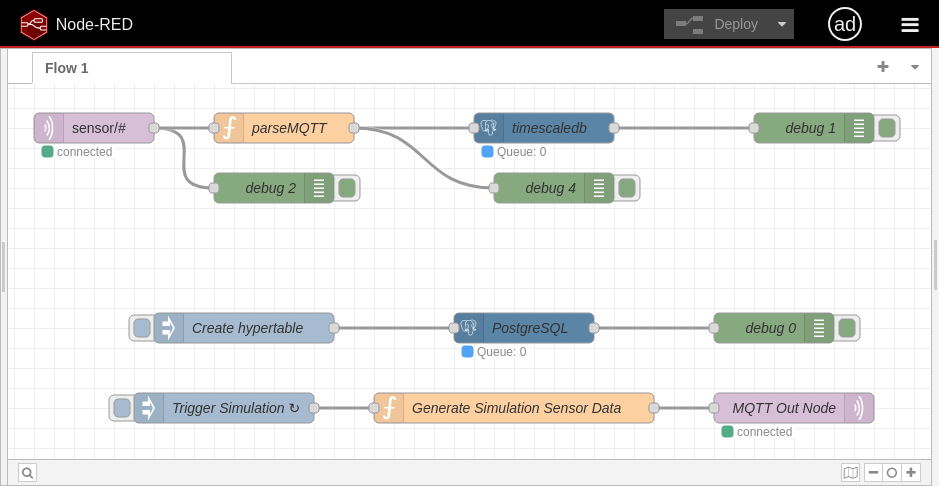
\includegraphics[width=0.85\textwidth]{imgs/nodered.png}
  \caption{Lógica de procesamiento de datos implementada en Node-RED.}
  \label{fig:nodered_flows}
\end{figure}

\subsubsection{Visualización con Grafana}

La interfaz final de usuario se desarrolló sobre \textbf{Grafana}, permitiendo una visualización dinámica y en tiempo real de los parámetros eléctricos:

\begin{itemize}
  \item \textbf{Dashboard Principal:} Muestra variables críticas como potencia activa total, tensiones de fase, corrientes y energía acumulada.
  \item \textbf{Análisis Histórico:} Permite al usuario comparar consumos y generación fotovoltaica a lo largo de diferentes períodos de tiempo (día, semana, mes).
  \item \textbf{Responsive Design:} El dashboard es accesible desde navegadores web y dispositivos móviles, adaptándose automáticamente al tamaño de pantalla.
  \item \textbf{Gestión de Usuarios y Control de Acceso:} Se utiliza el sistema de autenticación de Grafana para gestionar diferentes niveles de permisos. Esta capacidad es clave para la empresa, ya que permite aislar los dashboards de cada cliente, asegurando que cada usuario final visualice únicamente la información perteneciente a su instalación fotovoltaica.
\end{itemize}

\begin{figure}[H]
  \centering
  \fbox{
    \begin{minipage}{0.6\textwidth} \centering \vspace{2cm} [Captura de pantalla: Dashboard Principal de Grafana] \vspace{2cm}
  \end{minipage}}
  \caption{Interfaz de usuario para el monitoreo de la instalación trifásica.}
  \label{fig:grafana_dashboard}
\end{figure}

\subsection{Ensayos y Resultados}

\subsubsection{Implementación del prototipo}

En esta sección se presenta la materialización física del sistema, desde el ensamble de la placa de circuito impreso hasta la integración final en su gabinete.

\begin{figure}[H]
  \centering
  \fbox{
    \begin{minipage}{0.6\textwidth} \centering \vspace{2cm} [Fotografía: PCB físico ensamblado y en funcionamiento] \vspace{2cm}
  \end{minipage}}
  \caption{Implementación física del prototipo final sobre circuito impreso.}
  \label{fig:pcb_fisico}
\end{figure}

\begin{figure}[H]
  \centering
  \fbox{
    \begin{minipage}{0.8\textwidth} \centering \vspace{3cm} [Fotografía: Prototipo completo en su presentación final] \vspace{3cm}
  \end{minipage}}
  \caption{Prototipo final del medidor trifásico bidireccional listo para su instalación.}
  \label{fig:prototipo_final}
\end{figure}

\begin{table}[htbp]
  \centering
  \caption{Listado de componentes para la fabricación del prototipo.}
  \label{tab:componentes}
  \begin{tblr}{
      colspec = {X[l] c},
      hlines, vlines,
      row{1} = {bg=azure7, font=\bfseries},
    }
    Componente                                                   & Cantidad \\
    Microcontrolador STM32F103 --- \textit{Blue Pill} DevBoard   & 1        \\
    Módulo ESP32-C3 SuperMini (Gateway IoT)                      & 1        \\
    Transformador de tensión ZMPT101B                            & 3        \\
    Potenciómetro digital MCP4131                                & 3        \\
    Amplificador operacional LMV324                              & 2        \\
    Fuente de alimentación switching HLK-5M05                   & 1        \\
    Varistor de protección                                       & 1        \\
    Fusible 5$\times$20\,mm con portafusible                     & 1        \\
    Resistor 820\,k$\Omega$                                      & 3        \\
    Resistor 33\,$\Omega$                                        & 3        \\
    Resistor 10\,k$\Omega$                                       & 6        \\
    Resistor 3{,}3\,k$\Omega$                                    & 3        \\
    Resistor 5{,}1\,k$\Omega$                                    & 2        \\
    Capacitor 100\,nF                                            & 5        \\
    Capacitor electrolítico 10\,$\mu$F                           & 1        \\
    Conector jack 3.5\,mm 4 pines --- entrada SCT-013            & 3        \\
    Bloque de terminales 4P paso 5\,mm --- entrada red           & 1        \\
    Conector Molex KK 2P --- salida alimentación                 & 1        \\
    Conectores varios (pin headers y jumpers)                    & 23       \\
    Tornillos de fijación M3                                     & 4        \\
    Circuito impreso (PCB)                                       & 1        \\
  \end{tblr}
\end{table}

La tabla \ref{tab:componentes} detalla el listado de componentes utilizados para la construcción del dispositivo. El costo total de implementación se estima en aproximadamente ARS [Suma Final]. Este valor refleja la inversión necesaria para la construcción de una unidad funcional como prototipo, considerando precios minoristas y costos de adquisición en el mercado local a la fecha de escritura. En una etapa de producción seriada, el costo por unidad se vería reducido por la optimización de procesos y compras por volumen.

\subsubsection{Pruebas de Exactitud y Linealidad}

\section{Vinculación de las tareas/proyectos con Asignaturas de la Carrera}

El desarrollo de este proyecto integra conocimientos de diversas áreas de la Ingeniería en Computación, permitiendo la aplicación práctica de conceptos teóricos en un entorno de diseño real:

\begin{itemize}
  \item \textbf{Sistemas Embebidos / Arquitectura de Computadoras / Procesamiento de Señales:} El uso de microcontroladores STM32 y ESP32 requirió el manejo de periféricos avanzados como ADC con DMA, temporizadores para muestreo preciso e interrupciones. La implementación de algoritmos para el cálculo de RMS y potencia activa se vincula directamente con el procesamiento digital de señales.
  \item \textbf{Redes / Internet de las Cosas:} La implementación de la pila IoT involucró el uso de protocolos de transporte como TCP/IP y protocolos de aplicación como MQTT. La seguridad fue un factor clave, aplicando cifrado TLS para proteger la integridad de los datos en un entorno conectado.
  \item \textbf{Circuitos Eléctricos:} El cálculo de parámetros como el valor eficaz (RMS) de tensión y corriente, la potencia activa mediante integración numérica y el factor de potencia se basa directamente en los fundamentos teóricos de esta asignatura.
  \item \textbf{Programación / Algoritmos y Estructuras de Datos:} El desarrollo del firmware en C/C++ exigió la aplicación de buenas prácticas de programación, gestión de memoria eficiente y el uso de protocolos de comunicación serial.
\end{itemize}

\section{Equipamiento y Herramientas utilizadas}

Para la realización de esta práctica se utilizaron las siguientes herramientas y componentes tecnológicos:

\begin{itemize}
  \item \textbf{Instrumental de Laboratorio:}
    \begin{itemize}
      \item \textbf{Osciloscopio Digital:} Utilizado para la visualización de las formas de onda de tensión y corriente, verificación de la integridad de las señales acondicionadas y medición precisa de los tiempos de retardo de fase.
      \item \textbf{Multímetro Digital:} Empleado para la calibración de los sensores y la verificación de niveles de tensión en las etapas de alimentación y acondicionamiento.
      \item \textbf{Fuente de Alimentación Regulada:} Utilizada para el suministro de energía a las etapas analógicas y digitales durante las pruebas de prototipado.
      \item \textbf{Estación de Soldadura y Herramientas de Prototipado:} Para el montaje del hardware en placas de desarrollo y circuitos impresos experimentales.
    \end{itemize}
  \item \textbf{Componentes de Hardware del Sistema:}
    \begin{itemize}
      \item Microcontroladores STM32F103 (medición) y ESP32-C3 (comunicaciones).
      \item Potenciómetros digitales MCP4131 y amplificadores operacionales LMV324.
      \item Sensores de corriente SCT-013 y transformadores ZMPT101B.
    \end{itemize}
  \item \textbf{Entornos de Desarrollo y Software:}
    \begin{itemize}
      \item Visual Studio Code (con extensiones STM32 y PlatformIO).
      \item \textbf{KiCad EDA:} Para el diseño del esquemático y el ruteo del circuito impreso.
      \item Docker y Docker Compose para el despliegue de la infraestructura remota.
      \item Grafana y Node-RED para la visualización y orquestación de datos.
    \end{itemize}
\end{itemize}

\section{Conclusiones}

La realización de esta Práctica Profesional Supervisada permitió consolidar los conocimientos adquiridos durante la carrera mediante el desarrollo de un sistema embebido complejo que integra hardware, firmware y servicios de conectividad. El diseño basado en una arquitectura dual (STM32 + ESP32) demostró ser una solución robusta y eficiente, permitiendo delegar las tareas críticas de medición a un microcontrolador dedicado con capacidades de procesamiento en tiempo real, mientras que la gestión de la conectividad y la seguridad IoT fue resuelta por un procesador especializado en redes.

La implementación del sistema de ajuste automático de rango (\textit{auto-ranging}) representó uno de los mayores desafíos y logros técnicos del proyecto. Este mecanismo permitió extender significativamente el rango dinámico del medidor, garantizando la exactitud en mediciones de hasta \SI{70}{\ampere} RMS. Esto lo posiciona como una solución sumamente versátil para el monitoreo de instalaciones residenciales y comerciales donde las variaciones de carga y generación pueden ser muy amplias a lo largo del día.

Asimismo, el enfoque centrado en la seguridad mediante el uso de protocolos cifrados (MQTTS/TLS) y la flexibilidad otorgada por la gestión dinámica de credenciales WiFi posicionan a este prototipo como una base sólida para un producto comercial escalable y confiable.

Como trabajo futuro, se contempla la posibilidad de migrar la etapa de adquisición de señales hacia circuitos integrados especializados en medición de energía (\textit{AFE - Analog Front End}) como los de la familia MCP3903/MCP3913. La utilización de estos integrados simplificaría notablemente el diseño del hardware al integrar convertidores de alta resolución y funciones de cálculo nativas, facilitando la producción a escala del dispositivo. Cabe destacar que, si bien se evaluó esta opción, se optó por la solución discreta actual basada en el STM32 debido a la escasa disponibilidad de dichos integrados especializados al momento de la ejecución del proyecto.

\nocite{*}
\printbibliography[heading=bibnumbered,title=Bibliografía]

\appendix

\section{Código Fuente y Repositorios}

Todo el material desarrollado para este proyecto, incluyendo el firmware de los microcontroladores, la configuración de la infraestructura de servicios y los archivos de diseño del hardware, se encuentra alojado en repositorios públicos de GitHub. La organización del código sigue una estructura modular para facilitar su mantenimiento y escalabilidad:

\begin{itemize}
  \item \textbf{Firmware STM32:} Contiene la lógica de adquisición ADC, procesamiento de señales y algoritmos de cálculo RMS. \\ \url{https://github.com/fabcontigiani/stm32-pps-enerlab}

  \item \textbf{Firmware ESP32:} Incluye la gestión de conectividad WiFiManager, comunicación MQTTS, portal cautivo y diagnósticos locales. \\ \url{https://github.com/fabcontigiani/esp32-pps-enerlab}

  \item \textbf{Infraestructura Docker (Servicios Remotos):} Orquestación de contenedores para TimescaleDB, Grafana, Node-RED y Mosquitto. \\ \url{https://github.com/fabcontigiani/docker-pps-enerlab}

  \item \textbf{Proyecto KiCad (Hardware y PCB):} Archivos de diseño esquemático, ruteo del PCB y modelos 3D del hardware. \\ \url{https://github.com/fabcontigiani/kicad-pps-enerlab}
\end{itemize}
\section{Manual de Usuario y Guía Técnica}

Este anexo proporciona las directrices necesarias para la correcta instalación física del dispositivo, su configuración lógica y el despliegue de la infraestructura de backend por parte del personal de la empresa.

\subsection{Guía de Instalación y Conexión Eléctrica}

Para asegurar la exactitud de las mediciones, el dispositivo debe conectarse siguiendo el esquema de fases de la instalación fotovoltaica:

\begin{enumerate}
  \item \textbf{Sensores de Corriente (SCT-013):} Deben abrazar los conductores de fase antes de la entrada al tablero principal. Es fundamental respetar la dirección de la flecha grabada en el sensor (apuntando hacia la carga) para evitar lecturas de potencia invertidas.
  \item \textbf{Conexión de Tensión y Neutro:} El dispositivo cuenta con un conector para las tres fases y el neutro. No se requiere cableado adicional para los transformadores internos, basta con insertar el conector correspondiente asegurando un contacto firme para una medición de tensión segura.
  \item \textbf{Alimentación:} El medidor es un sistema autónomo que se alimenta directamente de la Fase 1, no se requiere de una fuente de alimentación externa adicional, ya que el hardware integra su propia etapa de alimentación.
\end{enumerate}

\begin{figure}[H]
  \centering
  \fbox{
    \begin{minipage}{0.6\textwidth} \centering \vspace{2cm} [Esquema/Fotografía: Conexión de sensores y alimentación] \vspace{2cm}
  \end{minipage}}
  \caption{Diagrama de conexión física del medidor en el tablero eléctrico.}
  \label{fig:manual_instalacion}
\end{figure}

\subsection{Configuración Inicial del Dispositivo}

Una vez energizado por primera vez, el medidor entrará en modo de configuración automática:

\begin{enumerate}
  \item \textbf{Conexión al AP:} Desde un dispositivo móvil o PC, buscar la red Wi-Fi denominada \texttt{Enerlab WiFiManager} e ingresar la clave \texttt{password}, la cual es configurable en el código fuente y puede ser modificada por la empresa.
  \item \textbf{Portal Cautivo:} Al conectarse, se abrirá automáticamente un portal web. En caso de que esto no ocurra, navegar a \url{http://enerlab.local} o a la dirección IP \texttt{192.168.4.1}.
  \item \textbf{Configuración de Red:} Seleccionar la red Wi-Fi local, ingresar la contraseña y guardar. El dispositivo se reiniciará e intentará conectarse al broker MQTT configurado por defecto.
\end{enumerate}

El proceso de vinculación del dispositivo a la red Wi-Fi local se detalla gráficamente en la figura~\ref{fig:portal_wifi_config} (página~\pageref{fig:portal_wifi_config}).

\subsection{Monitoreo y Diagnóstico Local}

El usuario o instalador puede acceder a la interfaz de diagnóstico local ingresando \url{http://enerlab.local} o la dirección IP asignada al medidor en su navegador. Esta interfaz permite:
\begin{itemize}
  \item Visualizar el estado de la comunicación con el broker MQTT.
  \item Verificar las versiones de firmware instaladas.
  \item Consultar los \textit{logs} de errores en tiempo real almacenados en la memoria interna.
\end{itemize}

La pantalla de estado y diagnóstico accesible vía mDNS se ilustra en la figura~\ref{fig:web_monitoreo} (página~\pageref{fig:web_monitoreo}).

\subsection{Guía para la Empresa: Despliegue de Servicios y Gestión}

El despliegue del backend se realiza de forma centralizada mediante Docker, siguiendo un flujo de trabajo que garantiza la seguridad y la portabilidad:

\begin{enumerate}
  \item \textbf{Preparación del Entorno:}
    \begin{itemize}
      \item Clonar el repositorio de infraestructura.
      \item Crear el archivo de configuración local: \texttt{cp .env.example .env}.
      \item Editar el archivo \texttt{.env} definiendo contraseñas robustas para la base de datos, secretos para Node-RED y ajustando la variable \texttt{TZ} a la zona horaria local.
    \end{itemize}
  \item \textbf{Configuración de Red y Dominio:}
    \begin{itemize}
      \item Definir el dominio base en el \texttt{.env} para que el servicio SWAG gestione automáticamente los certificados TLS.
      \item \textbf{Intervención Manual en Mosquitto:} Dado que el servicio de mensajería no soporta variables de entorno en su configuración nativa, se debe editar manualmente el archivo \texttt{mosquitto/config/mosquitto.conf} para actualizar las rutas de los certificados (\texttt{cafile}, \texttt{certfile}, \texttt{keyfile}) con el nombre del dominio seleccionado.
    \end{itemize}
  \item \textbf{Despliegue:} Ejecutar \texttt{docker-compose up -d}. Esto levantará automáticamente la base de datos TimescaleDB, el broker MQTT, Node-RED, Grafana y el proxy inverso.
  \item \textbf{Gestión de Usuarios en Grafana:}
    \begin{itemize}
      \item Acceder al panel de administración de Grafana.
      \item Crear \textit{Organizations} independientes para cada cliente.
      \item Asignar usuarios con rol de \textit{Viewer} a sus respectivas organizaciones para asegurar que solo tengan acceso a sus \textit{dashboards}, manteniendo la privacidad de la información entre clientes de la empresa. Para más detalles sobre la configuración avanzada, consultar la documentación oficial de Grafana sobre \href{https://grafana.com/docs/grafana/latest/administration/user-management/}{gestión de usuarios}, \href{https://grafana.com/docs/grafana/latest/administration/roles-and-permissions/}{roles y permisos}.
    \end{itemize}
\end{enumerate}

\section{Capturas del Diseño de PCB}
\label{sec:anexo_pcb}


En esta sección se presentan las capturas detalladas del diseño del circuito impreso (PCB) realizado en KiCad, incluyendo el ruteado de pistas, la disposición de componentes y vistas en tres dimensiones. El proyecto completo con los archivos fuente se encuentra disponible en el repositorio de KiCad compartido anteriormente (\url{https://github.com/fabcontigiani/kicad-pps-enerlab}).


\begin{figure}[H]
  \centering
  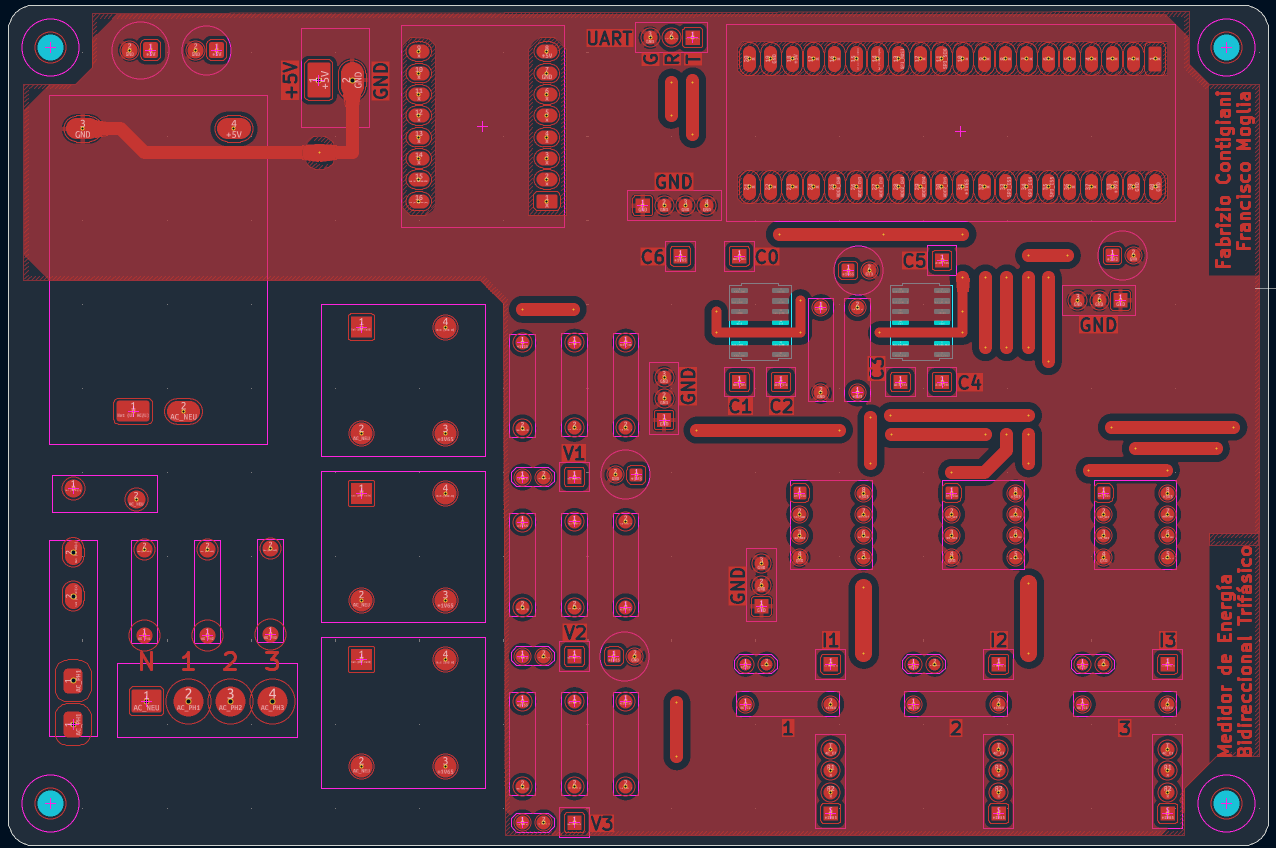
\includegraphics[width=0.8\textwidth]{imgs/capa_superior_kicad.png}
  \caption{Ruteado de la capa superior (Top Layer) de la PCB.}
  \label{fig:anexo_pcb_top}
\end{figure}

\begin{figure}[H]
  \centering
  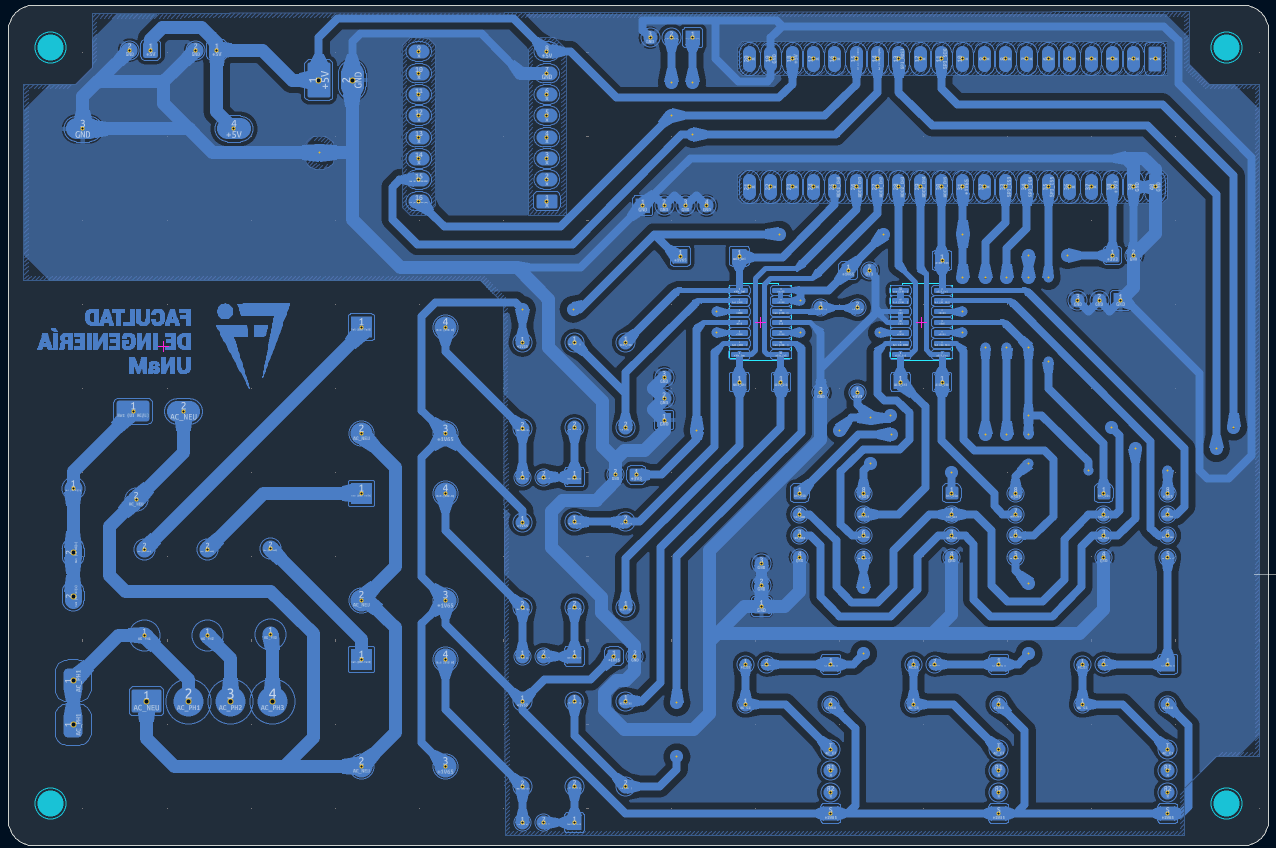
\includegraphics[width=0.8\textwidth]{imgs/capa_inferior_kicad.png}
  \caption{Ruteado de la capa inferior (Bottom Layer) de la PCB.}
  \label{fig:anexo_pcb_bottom}
\end{figure}

\begin{figure}[H]
  \centering
  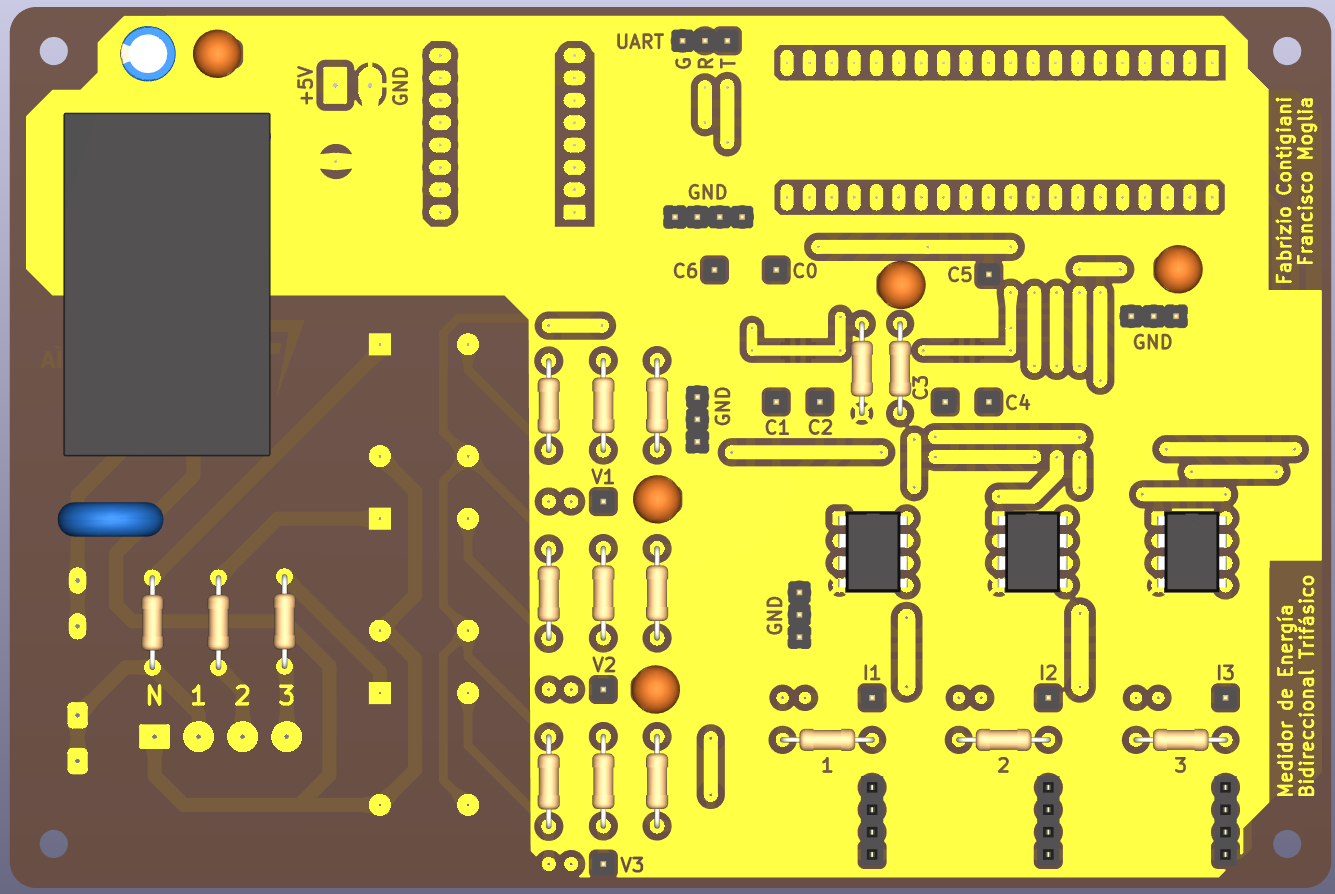
\includegraphics[width=0.8\textwidth]{imgs/vista_3d_kicad.png}
  \caption{Renderizado 3D detallado de la placa ensamblada.}
  \label{fig:anexo_pcb_3d}
\end{figure}

\end{document}